\documentclass{article}
\usepackage{graphicx}
\usepackage{array,color}
\usepackage{fancyhdr}
\usepackage{extramarks}
\usepackage{extramarks}
\usepackage{amsmath}
\usepackage{amsthm}
\usepackage{amsfonts}
\usepackage{tikz}
\usepackage[plain]{algorithm}
\usepackage{algpseudocode}
\usepackage{indentfirst}
\usepackage{amssymb}
\usepackage{mdwtab}
\usepackage{multirow}
\usepackage{booktabs}
\usepackage{dcolumn}
\usepackage{pdfpages}
\usepackage{calrsfs}
\usepackage[round]{natbib}
\usepackage[nottoc,numbib]{tocbibind}
\usepackage{hyperref}
\usepackage{rotating}
\usepackage{amssymb}
\usepackage{graphicx}
\usepackage{unicode-math}
\setlength{\parindent}{2em}
\usetikzlibrary{automata,positioning}

\usepackage[utf8]{inputenc}

\usepackage{listings}
\usepackage{xcolor}

\definecolor{codegreen}{rgb}{0,0.6,0}
\definecolor{codegray}{rgb}{0.5,0.5,0.5}
\definecolor{codepurple}{rgb}{0.58,0,0.82}
\definecolor{backcolour}{rgb}{0.95,0.95,0.92}

\lstdefinestyle{mystyle}{
	backgroundcolor=\color{backcolour},   
	commentstyle=\color{codegreen},
	keywordstyle=\color{magenta},
	numberstyle=\tiny\color{codegray},
	stringstyle=\color{codepurple},
	basicstyle=\ttfamily\tiny,
	breakatwhitespace=false,         
	breaklines=true,                 
	captionpos=b,                    
	keepspaces=true,                 
	numbers=left,                    
	numbersep=5pt,                  
	showspaces=false,                
	showstringspaces=false,
	showtabs=false,                  
	tabsize=2,
	rulecolor=\color{black}
}

\lstset{style=mystyle}

\renewcommand{\bibname}{References}

%
% Basic Document Settings
%

\topmargin=-0.45in
\evensidemargin=0in
\oddsidemargin=0in
\textwidth=6.5in
\textheight=9.0in
\headsep=0.25in

\linespread{1.5}

\pagestyle{fancy}
\lhead{\hmwkTitle}
\rhead{\hmwkClass}
\chead{\firstxmark}
\lfoot{\lastxmark}
\cfoot{\thepage}

\renewcommand\headrulewidth{0.4pt}
\renewcommand\footrulewidth{0.4pt}

\setlength\parindent{0pt}

%
% Homework Details
%   - Title
%   - Class
%   - Section/Time
%   - Instructor
%   - Author
%

\newcommand{\hmwkTitle}{Paper Replication with R}
\newcommand{\hmwkClass}{MIS7420 Seminar in Management Information Systems}
\newcommand{\hmwkClasstwo}{MIS7420 \\ Seminar in Management Information Systems}
\newcommand{\hmwkClassInstructor}{Prof. Zhiqiang Zheng, Prof. Vijay Mookerjee }
\newcommand{\hmwkAuthorName}{\textbf{Author: Beyza Celik, Luoying Chen, Yihong Liu, Duc Vu }}
\newcommand{\hmwkID}{\textbf{NETID:  BXC190000, LXC190027, YXL180111, DDV110020}}
%
% Title Page
%

\DeclareMathAlphabet{\pazocal}{OMS}{zplm}{m}{n}
\newcommand{\La}{\mathcal{L}}
\newcommand{\Lb}{\pazocal{L}}

\title{
    \vspace{2in}
    \textmd{\textbf{\hmwkClasstwo:\ \\ \hmwkTitle}}\\
    \vspace{1in}\large{\textit{\hmwkClassInstructor}}
    \vspace{2in}
}

\author{\hmwkAuthorName
\  \\ \hmwkID
\vspace{0.3in}}

\date{}

\renewcommand{\part}[1]{\textbf{\large Part \Alph{partCounter}}\stepcounter{partCounter}\\}

\renewcommand*{\lstlistingname}{Code}
\renewcommand*{\lstlistlistingname}{List of Codes}
%\captionsetup[lstlisting]{margin=0cm,format=hang,font=small,format=plain,labelfont={bf,up},textfont={it}}
%\captionsetup[lstlistoflistings]{\lstname Code \arabic{lstlisting} :}

\begin{document}

\maketitle

\pagebreak

% Make Table of Contents
\tableofcontents
\pagebreak
% Make List of Figures
\listoffigures
\pagebreak
% Make List of Tables
\listoftables
\pagebreak
% Make List of Codes
\addcontentsline{toc}{section}{List of Codes}
\lstlistoflistings 
\pagebreak

\section{Data Cleaning Process}
In this section, we present our codes for data cleaning and panel data preparation. Package \texttt{dplyr} \cite{wickham2015dplyr}, \texttt{haven} \cite{wickham2018haven}, \texttt{sqldf} \cite{grothendieck2017sqldf}, \texttt{zoo} \cite{zeileis2005zoo}, \texttt{plm} \cite{croissant2008panel}, are used in this process. \\
Notice that the provided data only contain users' browsing transactions with purchase. When we apply search engine filter on reference domain, besides google.com, yahoo.com, bing.com, some other search engines (msn.com, aol.com, live.com, mywebsearch.com) and five vendors (amazon.com, staples.com, dell.com, walmart.com, bestbuy.com) are also involved. For product categories, we only consider those sold at Circuit City and exclude three other types (Business machines, Office furniture, Office supplies
).\\
% Focused Variables
For \texttt{CCStorePresent}, its value is the same as \texttt{Store\_Close\_Status} in original data. And we set \texttt{AfterStoreClosing} to 0 if the time of user transaction is before November, 2008 and 1 otherwise. For \texttt{BBStorePresent}, we set it as 1 for user transactions if there's any Best Buy stores around user's location and 0 otherwise, using the \texttt{bestbuyzipcodes\_sample} dataset. \texttt{NoReferringDomain} is the variable we construct if the user directly came to the target website without any referring domain. And \texttt{ReferringDomainIsSearchEngine} is the variable we construct if the user was referred by search engine to the target website.\\
Finally, two panel data are constructed by concatenating \texttt{sales\_allotherzipcode} with \texttt{sales\_ccity0mile} and \texttt{sales\_ccity5mile}. After the concatenation and aggregation, we found that the built panel data are unbalanced, in a sense that, for instance, \texttt{zip\_code} 75080 only has 2 records, instead of 24 (2 years). It happens because (a) the provided data are a small sample from the whole original one; (b) the original data might not cover the full 2 years period. Unbalanced panel data has been studied by many researchers \cite{baltagi2006unbalanced}, like unbalanced seemingly unrelated regression \cite{mcdowell2004help}. Here we adopt a naive solution: we impute the missing values for one \texttt{zip\_code} by averaging those non-missing values of this \texttt{zip\_code}.
% imbalanced Panel Data
%\lstinputlisting[language=R, caption={Data Preprocess}, label={lst:dtaclean}, linerange={1-7, 10-63, 71-134, 138-143}]{../data_clean.R}

\pagebreak

\section{Paper Replication}
In this section, we provide our replication for this paper. Names for subsections correspond to the tables in the published paper. Package \texttt{stargazer} \cite{hlavac2015stargazer} and \texttt{estout} \cite{jann2004estout} are used to export estimation into \LaTeX \ format.
\subsection{Table 1}
Table \ref{tab:table1} shows the summary statistics of top five vendors by sales volume.
\begin{table}[!h] \centering 
	\caption{Summary Statistics of Top Five Vendors by Sales Volume} 
	\label{tab:table1} 
	\resizebox{\columnwidth}{!}{
		\begin{tabular}{@{\extracolsep{5pt}} D{.}{.}{-3} D{.}{.}{-3} D{.}{.}{-3} D{.}{.}{-3} D{.}{.}{-3} D{.}{.}{-3} D{.}{.}{-3} } 
			\\[-1.8ex]\hline 
			\hline 
			%\\[-1.8ex] 
			\multicolumn{1}{c}{\textbf{\begin{tabular}[c]{@{}c@{}}Domain \\ Name\end{tabular}}} & \multicolumn{1}{c}{\textbf{\begin{tabular}[c]{@{}c@{}}Total \\ Transactions\end{tabular}}} & \multicolumn{1}{c}{\textbf{\begin{tabular}[c]{@{}c@{}}Total \\ Sales\end{tabular}}} & \multicolumn{1}{c}{\textbf{\begin{tabular}[c]{@{}c@{}}Total Pages \\ Viewed\end{tabular}}} & \multicolumn{1}{c}{\textbf{\begin{tabular}[c]{@{}c@{}}Pages \\ Per Dollar\end{tabular}}} & \multicolumn{1}{c}{\textbf{\begin{tabular}[c]{@{}c@{}}Total \\ Duration\end{tabular}}} & \multicolumn{1}{c}{\textbf{\begin{tabular}[c]{@{}c@{}}Mins \\ Per Dollar\end{tabular}}} \\ 
			\hline \\[-1.8ex] 
			\multicolumn{1}{c}{dell.com} & 1,620 & 483,703.300 & 66,953 & 0.138 & 57,225.660 & 0.118 \\ 
			\multicolumn{1}{c}{amazon.com} & 10,904 & 354,573.300 & 464,383 & 1.310 & 369,227.900 & 1.041 \\ 
			\multicolumn{1}{c}{staples.com} & 5,927 & 236,982.300 & 247,163 & 1.043 & 166,189.900 & 0.701 \\ 
			\multicolumn{1}{c}{walmart.com} & 1,977 & 156,606.100 & 80,397 & 0.513 & 68,434.890 & 0.437 \\ 
			\multicolumn{1}{c}{bestbuy.com} & 1,230 & 149,950.400 & 50,627 & 0.338 & 36,735.900 & 0.245 \\ 
			\bottomrule
			%\hline \\[-1.8ex] 
		\end{tabular} 
	}
\end{table}

Codes for generating Table \ref{tab:table1} are listed below.
%\lstinputlisting[language=R, caption={Table 1 Generation}, label={lst:table1}, linerange={228-231}]{../data_clean.R}

\pagebreak
\subsection{Table 2}
Table \ref{tab:table2} summarizes the frequency of referral channels for various online retailers.
\begin{table}[!h] \centering 
	\caption{Summary Statistics of Referring Domain Categories} 
	\label{tab:table2} 
	\resizebox{\columnwidth}{!}{
		\begin{tabular}{@{\extracolsep{5pt}} D{.}{.}{-3} D{.}{.}{-3} D{.}{.}{-3} D{.}{.}{-3} D{.}{.}{-3} } 
			\\[-1.8ex]\hline 
			\hline 
			%\\[-1.8ex] 
			\multicolumn{1}{c}{\textbf{\begin{tabular}[c]{@{}c@{}}Domain \\ Name\end{tabular}}} & \multicolumn{1}{c}{\textbf{\begin{tabular}[c]{@{}c@{}}Total \\ Transactions\end{tabular}}} & \multicolumn{1}{c}{\textbf{\begin{tabular}[c]{@{}c@{}}Referred by \\ Search Engine\end{tabular}}} & \multicolumn{1}{c}{\textbf{\begin{tabular}[c]{@{}c@{}}Direct to \\ Website\end{tabular}}} & \multicolumn{1}{c}{\textbf{\begin{tabular}[c]{@{}c@{}}Referred by \\ Others\end{tabular}}} \\ 
			\hline \\[-1.8ex]  
			\multicolumn{1}{c}{amazon.com} & 10,904 & 2,955(27.1\%) & 7,018(64.4\%) & 931(8.6\%) \\ 
			\multicolumn{1}{c}{bestbuy.com} & 1,230 & 258(21.0\%) & 901(73.3\%) & 71(5.8\%) \\ 
			\multicolumn{1}{c}{All Others} & 36,794 & 6,999(19.0\%) & 25,483(69.3\%) & 4,312(11.7\%) \\ 
			\multicolumn{1}{c}{All Transactions} & 48,928 & 10,212(20.9\%) & 33,402(68.3\%) & 5,314(10.9\%) \\
			\bottomrule
			%\hline \\[-1.8ex] 
		\end{tabular} 
	}
\end{table}

Codes for generating Table \ref{tab:table2} are listed below.
%\lstinputlisting[language=R, caption={Table 2 Generation}, label={lst:table2}, linerange={233-239}]{../data_clean.R}

\pagebreak
\subsection{Table 3}
Table \ref{tab:table3} reports the model-free average DID values for some outcome variables.
\begin{table}[!h]
	\centering
	\caption{Average Difference-in-Difference (DID) of the Outcome Variables}
	\label{tab:table3}
	\scalebox{0.8}{
		\begin{tabular}{@{}cccccc@{}}
			\\[-1.8ex]\hline 
			\hline 
			%\\[-1.8ex] 
			\textbf{Outcome Variable} &
			\textbf{Groups} &
			\begin{tabular}[c]{@{}c@{}}\textbf{After Store}\\ \textbf{Closure}\end{tabular} &
			\begin{tabular}[c]{@{}c@{}}\textbf{Before Store}\\ \textbf{Closure}\end{tabular} &
			\begin{tabular}[c]{@{}c@{}}\textbf{First Difference} \\ (se)\end{tabular} &
			\textbf{DID} \\ \midrule
			\multirow{2}{*}{\begin{tabular}[c]{@{}c@{}}Amazon\\ Sales\end{tabular}} &
			Control & 3.418 & 3.303 &
			\begin{tabular}[c]{@{}c@{}}0.115\\ (0.031)\end{tabular} &
			\multirow{2}{*}{-0.167} \\ 	& Treatment & 3.351 & 3.403 &
			\begin{tabular}[c]{@{}c@{}}-0.052\\ (0.212)\end{tabular} & \\
			\multirow{2}{*}{\begin{tabular}[c]{@{}c@{}}Amazon\\ PagesPerDollar\end{tabular}} &
			Control & 1.188 & 1.147 &
			\begin{tabular}[c]{@{}c@{}}0.041\\ (0.025)\end{tabular} &
			\multirow{2}{*}{0.257} \\ & Treatment & 1.363 & 1.065 &
			\begin{tabular}[c]{@{}c@{}}0.298\\ (0.153)\end{tabular} & \\
			\multirow{2}{*}{\begin{tabular}[c]{@{}c@{}}Amazon\\ MinsPerDollar\end{tabular}} &
			Control & 1.016 & 0.975 &
			\begin{tabular}[c]{@{}c@{}}0.041\\ (0.025)\end{tabular} &
			\multirow{2}{*}{0.263} \\ & Treatment & 1.187 & 0.882 &
			\begin{tabular}[c]{@{}c@{}}0.304\\ (0.137)\end{tabular} &
			\\ \multirow{2}{*}{\begin{tabular}[c]{@{}c@{}}bestbuy.com\\ Sales\end{tabular}} &
			Control & 3.418 & 3.303 &
			\begin{tabular}[c]{@{}c@{}}0.354\\ (0.031)\end{tabular} &
			\multirow{2}{*}{0.623} \\ & Treatment & 3.351 & 3.403 &
			\begin{tabular}[c]{@{}c@{}}0.976\\ (0.212)\end{tabular} &
			\\ \multirow{2}{*}{\begin{tabular}[c]{@{}c@{}}bestbuy.com\\ PagesPerDollar\end{tabular}} &
			Control & 1.188 & 1.147 &
			\begin{tabular}[c]{@{}c@{}}-0.109\\ (0.025)\end{tabular} &
			\multirow{2}{*}{0.074} \\ & Treatment & 1.363 & 1.065 &
			\begin{tabular}[c]{@{}c@{}}-0.035\\ (0.153)\end{tabular} &
			\\ \multirow{2}{*}{\begin{tabular}[c]{@{}c@{}}bestbuy.com\\ MinsPerDollar\end{tabular}} &
			Control & 1.016 & 0.975 &
			\begin{tabular}[c]{@{}c@{}}-0.084\\ (0.025)\end{tabular} &
			\multirow{2}{*}{-0.012} \\ & Treatment & 1.187 & 0.882 &
			\begin{tabular}[c]{@{}c@{}}-0.096\\ (0.137)\end{tabular} &
			\\ \bottomrule
		\end{tabular}
	}
\end{table}

Codes for generating Table \ref{tab:table3} are listed below.
%\lstinputlisting[language=R, caption={Table 3 Generation}, label={lst:table3}, linerange={15-15, 23-175}]{../table3.R}

\pagebreak
\subsection{Table 4}
In order to examine whether a competing online retailer benefits from the presence of a local showroom, we run the following regressions for Amazon.com and BestBuy.com:
\begin{equation}
	\begin{aligned}
		& \log\left( \texttt{TotalMonthlySales} + 1\right)_{i,t} \\ &= \mu_{i} + \tau_{t} 
		\\ &+ \beta_1 \ \texttt{CCStorePresent}_i \times \texttt{AfterStoreClosing}_t 
		\\ &+ \beta_2 \ \texttt{CCStorePresent}_i \times \texttt{AfterStoreClosing}_t \times \texttt{BBStorePresent}_i \\ & + \epsilon_{i,t}
	\end{aligned}
\end{equation}
\begin{table}[!h] \centering 
	\caption{Results of the Sales Effect (All Product Categories)} 
	\label{tab:table4} 
	\resizebox{0.8\columnwidth}{!}{
		\begin{tabular}{@{\extracolsep{1pt}}lD{.}{.}{-3} D{.}{.}{-3} D{.}{.}{-3} D{.}{.}{-3} } 
			\\[-1.8ex]\hline 
			\hline \\[-1.8ex] 
			% & \multicolumn{4}{c}{\textit{Dependent variable:}} \\ 
			% \cline{2-5} 
			% \\[-1.8ex] 
			& \multicolumn{4}{c}{log(TotalMonthlySales + 1)} \\ 
			& \multicolumn{1}{c}{Amazon-0 Mile} & \multicolumn{1}{c}{Amazon-5 Miles} & \multicolumn{1}{c}{BestBuy-0 Mile} & \multicolumn{1}{c}{BestBuy-5 Miles} \\ 
			\\[-1.8ex] & \multicolumn{1}{c}{(1)} & \multicolumn{1}{c}{(2)} & \multicolumn{1}{c}{(3)} & \multicolumn{1}{c}{(4)}\\ 
			\hline \\[-1.8ex] 
			$\beta_1$ & 0.014 & -0.005 & -0.002 & -0.002 \\ 
			& (0.015) & (0.008) & (0.033) & (0.008) \\ 
			$\beta_2$ & -0.033 & 0.003 & 0.009 & 0.002 \\ 
			& (0.022) & (0.010) & (0.036) & (0.010) \\ 
			\hline \\[-1.8ex] 
			Observations & \multicolumn{1}{c}{68,472} & \multicolumn{1}{c}{75,096} & \multicolumn{1}{c}{14,664} & \multicolumn{1}{c}{16,848} \\ 
			R$^{2}$ & \multicolumn{1}{c}{0.00003} & \multicolumn{1}{c}{0.00001} & \multicolumn{1}{c}{0.00002} & \multicolumn{1}{c}{0.00000} \\ 
			Adjusted R$^{2}$ & \multicolumn{1}{c}{-0.044} & \multicolumn{1}{c}{-0.044} & \multicolumn{1}{c}{-0.045} & \multicolumn{1}{c}{-0.045} \\ 
			F Statistic & \multicolumn{1}{c}{1.091 (df = 2; 65594)} & \multicolumn{1}{c}{0.278 (df = 2; 71942)} & \multicolumn{1}{c}{0.154 (df = 2; 14028)} & \multicolumn{1}{c}{0.035 (df = 2; 16121)} \\  
			\hline 
			\hline \\[-1.8ex] 
			\textit{Note:}  & \multicolumn{4}{r}{$^{*}$p$<$0.1; $^{**}$p$<$0.05; $^{***}$p$<$0.01} \\ 
		\end{tabular} 
	}
\end{table}

Codes for generating Table \ref{tab:table4} are listed below.
%\lstinputlisting[language=R, caption={Table 4 Generation}, label={lst:table4}, linerange={145-152, 248-252}]{../data_clean.R}

\pagebreak
\subsection{Table 5}
To measure the impact of the exit of local showrooms on consumer online
search intensity and the moderating effect of Best Buy Stores as an alternative local showroom, we run the following regressions:
\resizebox{.8\linewidth}{!}{
	\begin{minipage}{\linewidth}
		\begin{equation}
			\begin{aligned}
				& \log\left( \texttt{PagesPerDollar} + 1,\ \texttt{MinsPerDollar} + 1\right)_{i,t} \\ &= \mu_{i} + \tau_{t} 
				\\ &+ \beta_1 \ \texttt{CCStorePresent}_i \times \texttt{AfterStoreClosing}_t 
				\\ &+ \beta_2 \ \texttt{CCStorePresent}_i \times \texttt{AfterStoreClosing}_t \times \texttt{BBStorePresent}_i \\ & + \epsilon_{i,t}
			\end{aligned}
		\end{equation}
	\end{minipage}
}
\begin{table}[!htbp] \centering 
	\caption{Results of the Search Effect (All Product Categories)} 
	\label{tab:table5} 
	\resizebox{\columnwidth}{!}{
		\begin{tabular}{@{\extracolsep{1pt}}lD{.}{.}{-3} D{.}{.}{-3} D{.}{.}{-3} D{.}{.}{-3} D{.}{.}{-3} D{.}{.}{-3} D{.}{.}{-3} D{.}{.}{-3} } 
			\\[-1.8ex]\hline 
			\hline \\[-1.8ex] 
			%& \multicolumn{8}{c}{\textit{Dependent variable:}} \\ 
			%\cline{2-9} 
			%\\[-1.8ex] 
			& \multicolumn{4}{c}{log(PagesPerDollar + 1)} & \multicolumn{4}{c}{log(MinsPerDollar + 1)} \\ 
			& \multicolumn{1}{c}{Amazon-0 Mile} & \multicolumn{1}{c}{Amazon-5 Miles} & \multicolumn{1}{c}{BestBuy-0 Mile} & \multicolumn{1}{c}{BestBuy-5 Miles} & \multicolumn{1}{c}{Amazon-0 Mile} & \multicolumn{1}{c}{Amazon-5 Miles} & \multicolumn{1}{c}{BestBuy-0 Mile} & \multicolumn{1}{c}{BestBuy-5 Miles} \\ 
			\\[-1.8ex] & \multicolumn{1}{c}{(1)} & \multicolumn{1}{c}{(2)} & \multicolumn{1}{c}{(3)} & \multicolumn{1}{c}{(4)} & \multicolumn{1}{c}{(5)} & \multicolumn{1}{c}{(6)} & \multicolumn{1}{c}{(7)} & \multicolumn{1}{c}{(8)}\\ 
			\hline \\[-1.8ex] 
			$\beta_1$ & 0.003 & -0.019^{***} & 0.001 & 0.002 & 0.004 & -0.021^{***} & 0.001 & 0.003 \\ 
			& (0.012) & (0.007) & (0.016) & (0.004) & (0.012) & (0.007) & (0.013) & (0.003) \\ 
			$\beta_2$ & -0.068^{***} & 0.018^{**} & 0.003 & -0.001 & -0.057^{***} & 0.022^{***} & 0.0004 & -0.002 \\ 
			& (0.018) & (0.009) & (0.018) & (0.005) & (0.017) & (0.008) & (0.014) & (0.004) \\ 
			\hline \\[-1.8ex] 
			Observations & \multicolumn{1}{c}{68,472} & \multicolumn{1}{c}{75,096} & \multicolumn{1}{c}{14,664} & \multicolumn{1}{c}{16,848} & \multicolumn{1}{c}{68,472} & \multicolumn{1}{c}{75,096} & \multicolumn{1}{c}{14,664} & \multicolumn{1}{c}{16,848} \\ 
			R$^{2}$ & \multicolumn{1}{c}{0.0004} & \multicolumn{1}{c}{0.0001} & \multicolumn{1}{c}{0.00003} & \multicolumn{1}{c}{0.00004} & \multicolumn{1}{c}{0.0003} & \multicolumn{1}{c}{0.0001} & \multicolumn{1}{c}{0.00001} & \multicolumn{1}{c}{0.0001} \\ 
			Adjusted R$^{2}$ & \multicolumn{1}{c}{-0.043} & \multicolumn{1}{c}{-0.044} & \multicolumn{1}{c}{-0.045} & \multicolumn{1}{c}{-0.045} & \multicolumn{1}{c}{-0.044} & \multicolumn{1}{c}{-0.044} & \multicolumn{1}{c}{-0.045} & \multicolumn{1}{c}{-0.045} \\ 
			F Statistic & \multicolumn{1}{c}{12.530$^{***}$ (df = 2; 65594)} & \multicolumn{1}{c}{3.985$^{**}$ (df = 2; 71942)} & \multicolumn{1}{c}{0.202 (df = 2; 14028)} & \multicolumn{1}{c}{0.337 (df = 2; 16121)} & \multicolumn{1}{c}{8.867$^{***}$ (df = 2; 65594)} & \multicolumn{1}{c}{5.187$^{***}$ (df = 2; 71942)} & \multicolumn{1}{c}{0.046 (df = 2; 14028)} & \multicolumn{1}{c}{0.451 (df = 2; 16121)} \\ 
			\hline 
			\hline \\[-1.8ex] 
			\textit{Note:}  & \multicolumn{8}{r}{$^{*}$p$<$0.1; $^{**}$p$<$0.05; $^{***}$p$<$0.01} \\ 
		\end{tabular} 
	}
\end{table}

Codes for generating Table \ref{tab:table5} are listed below.
%\lstinputlisting[language=R, caption={Table 5 Generation}, label={lst:table5}, linerange={154-161, 278-283, 299-303}]{../data_clean.R}

\pagebreak
\subsection{Table 6}
To capture the expected change in the odds ratio of the impact of Circuit City store closures and
the moderating effect of Best Buy stores as an alternative local showroom, we run the following regressions:
\begin{equation}
	\begin{aligned}
		& \textrm{Logit}\left( \texttt{ReferringDomainIsSearchEngine}, \texttt{NoReferringDomain} \right)_{i,t} \\ &= \mu_{i} + \tau_{t} 
		\\ &+ \beta_1 \ \texttt{CCStorePresent}_i \times \texttt{AfterStoreClosing}_t 
		\\ &+ \beta_2 \ \texttt{CCStorePresent}_i \times \texttt{AfterStoreClosing}_t \times \texttt{BBStorePresent}_i \\ & + \epsilon_{i,t}
	\end{aligned}
\end{equation}
\begin{table}[!h] \centering 
	\caption{Results of the Sales Effect: Experience and Search Products} 
	\label{tab:table6} 
	\resizebox{\columnwidth}{!}{
	\begin{tabular}{@{\extracolsep{1pt}}lD{.}{.}{-3} D{.}{.}{-3} D{.}{.}{-3} D{.}{.}{-3} D{.}{.}{-3} D{.}{.}{-3} D{.}{.}{-3} D{.}{.}{-3} } 
		\\[-1.8ex]\hline 
		\hline \\[-1.8ex] 
		%& \multicolumn{8}{c}{\textit{Dependent variable:}} \\ 
		%\cline{2-9} 
		%\\[-1.8ex] 
		& \multicolumn{8}{c}{log(TotalMonthlySales + 1)} \\ 
		& \multicolumn{1}{c}{Amazon-0 Mile-Exp} & \multicolumn{1}{c}{Amazon-5 Miles-Exp} & \multicolumn{1}{c}{Amazon-0 Mile-Search} & \multicolumn{1}{c}{Amazon-5 Miles-Search} & \multicolumn{1}{c}{BestBuy-0 Mile-Exp} & \multicolumn{1}{c}{BestBuy-5 Miles-Exp} & \multicolumn{1}{c}{BestBuy-0 Mile-Exp} & \multicolumn{1}{c}{BestBuy-5 Miles-Search} \\ 
		\\[-1.8ex] & \multicolumn{1}{c}{(1)} & \multicolumn{1}{c}{(2)} & \multicolumn{1}{c}{(3)} & \multicolumn{1}{c}{(4)} & \multicolumn{1}{c}{(5)} & \multicolumn{1}{c}{(6)} & \multicolumn{1}{c}{(7)} & \multicolumn{1}{c}{(8)}\\ 
		\hline \\[-1.8ex] 
		$\beta_1$ & 0.005 & -0.007 & 0.005 & -0.008 & -0.011 & -0.009 & -0.001 & -0.010 \\ 
		& (0.017) & (0.010) & (0.013) & (0.006) & (0.009) & (0.007) & (0.023) & (0.008) \\ 
		$\beta_2$ & -0.043^{*} & 0.009 & -0.002 & 0.009 &  & 0.013 & 0.000 & 0.009 \\ 
		& (0.024) & (0.012) & (0.018) & (0.008) &  & (0.008) & (0.028) & (0.010) \\ 
		\hline \\[-1.8ex] 
		Observations & \multicolumn{1}{c}{32,112} & \multicolumn{1}{c}{35,568} & \multicolumn{1}{c}{52,392} & \multicolumn{1}{c}{57,648} & \multicolumn{1}{c}{10,224} & \multicolumn{1}{c}{11,712} & \multicolumn{1}{c}{5,664} & \multicolumn{1}{c}{6,600} \\ 
		R$^{2}$ & \multicolumn{1}{c}{0.0002} & \multicolumn{1}{c}{0.00002} & \multicolumn{1}{c}{0.00000} & \multicolumn{1}{c}{0.00003} & \multicolumn{1}{c}{0.0001} & \multicolumn{1}{c}{0.0002} & \multicolumn{1}{c}{0.00000} & \multicolumn{1}{c}{0.0002} \\ 
		Adjusted R$^{2}$ & \multicolumn{1}{c}{-0.044} & \multicolumn{1}{c}{-0.044} & \multicolumn{1}{c}{-0.044} & \multicolumn{1}{c}{-0.044} & \multicolumn{1}{c}{-0.046} & \multicolumn{1}{c}{-0.045} & \multicolumn{1}{c}{-0.048} & \multicolumn{1}{c}{-0.047} \\ 
		F Statistic & \multicolumn{1}{c}{2.775$^{*}$ (df = 2; 30749)} & \multicolumn{1}{c}{0.318 (df = 2; 34061)} & \multicolumn{1}{c}{0.101 (df = 2; 50184)} & \multicolumn{1}{c}{0.774 (df = 2; 55221)} & \multicolumn{1}{c}{1.377 (df = 1; 9774)} & \multicolumn{1}{c}{1.297 (df = 2; 11199)} & \multicolumn{1}{c}{0.004 (df = 2; 5403)} & \multicolumn{1}{c}{0.746 (df = 2; 6300)} \\ 
		\hline 
		\hline \\[-1.8ex] 
		\textit{Note:}  & \multicolumn{8}{r}{$^{*}$p$<$0.1; $^{**}$p$<$0.05; $^{***}$p$<$0.01} \\ 
\end{tabular} }
\end{table}

Codes for generating Table \ref{tab:table6} are listed below.
%\lstinputlisting[language=R, caption={Table 6 Generation}, label={lst:table6}, linerange={163-176, 332-341}]{../data_clean.R}

\pagebreak
\subsection{Table 7}
We then test whether the show-rooming effect is stronger for experience goods, by grouping products into physical experience goods and search goods. Table \ref{tab:table7} and \ref{tab:table8} presents the
results for sales model on physical experience products and search products separately.
\begin{table}[!h] \centering 
	\caption{Results of the Online Search Effect: Experience Products} 
	\label{tab:table7} 
	\resizebox{\columnwidth}{!}{
	\begin{tabular}{@{\extracolsep{1pt}}lD{.}{.}{-3} D{.}{.}{-3} D{.}{.}{-3} D{.}{.}{-3} D{.}{.}{-3} D{.}{.}{-3} D{.}{.}{-3} D{.}{.}{-3} } 
		\\[-1.8ex]\hline 
		\hline \\[-1.8ex] 
		%& \multicolumn{8}{c}{\textit{Dependent variable:}} \\ 
		%\cline{2-9} 
		%\\[-1.8ex] 
		& \multicolumn{4}{c}{log(PagesPerDollar + 1)} & \multicolumn{4}{c}{log(MinsPerDollar + 1)} \\ 
		& \multicolumn{1}{c}{Amazon-0 Mile} & \multicolumn{1}{c}{Amazon-5 Miles} & \multicolumn{1}{c}{BestBuy-0 Mile} & \multicolumn{1}{c}{BestBuy-5 Miles} & \multicolumn{1}{c}{Amazon-0 Mile} & \multicolumn{1}{c}{Amazon-5 Miles} & \multicolumn{1}{c}{BestBuy-0 Mile} & \multicolumn{1}{c}{BestBuy-5 Miles} \\ 
		\\[-1.8ex] & \multicolumn{1}{c}{(1)} & \multicolumn{1}{c}{(2)} & \multicolumn{1}{c}{(3)} & \multicolumn{1}{c}{(4)} & \multicolumn{1}{c}{(5)} & \multicolumn{1}{c}{(6)} & \multicolumn{1}{c}{(7)} & \multicolumn{1}{c}{(8)}\\ 
		\hline \\[-1.8ex] 
		$\beta_1$ & 0.007 & -0.037^{***} & 0.006^{**} & 0.001 & 0.006 & -0.039^{***} & 0.003 & 0.001 \\ 
		& (0.015) & (0.008) & (0.002) & (0.002) & (0.015) & (0.008) & (0.002) & (0.001) \\ 
		$\beta_2$ & -0.077^{***} & 0.030^{***} &  & -0.0001 & -0.067^{***} & 0.034^{***} &  & -0.001 \\ 
		& (0.020) & (0.010) &  & (0.002) & (0.020) & (0.010) &  & (0.002) \\ 
		\hline \\[-1.8ex] 
		Observations & \multicolumn{1}{c}{32,112} & \multicolumn{1}{c}{35,568} & \multicolumn{1}{c}{10,224} & \multicolumn{1}{c}{11,712} & \multicolumn{1}{c}{32,112} & \multicolumn{1}{c}{35,568} & \multicolumn{1}{c}{10,224} & \multicolumn{1}{c}{11,712} \\ 
		R$^{2}$ & \multicolumn{1}{c}{0.001} & \multicolumn{1}{c}{0.001} & \multicolumn{1}{c}{0.001} & \multicolumn{1}{c}{0.00003} & \multicolumn{1}{c}{0.001} & \multicolumn{1}{c}{0.001} & \multicolumn{1}{c}{0.0003} & \multicolumn{1}{c}{0.0001} \\ 
		Adjusted R$^{2}$ & \multicolumn{1}{c}{-0.043} & \multicolumn{1}{c}{-0.044} & \multicolumn{1}{c}{-0.045} & \multicolumn{1}{c}{-0.046} & \multicolumn{1}{c}{-0.044} & \multicolumn{1}{c}{-0.044} & \multicolumn{1}{c}{-0.046} & \multicolumn{1}{c}{-0.046} \\ 
		F Statistic & \multicolumn{1}{c}{12.857$^{***}$ (df = 2; 30749)} & \multicolumn{1}{c}{10.009$^{***}$ (df = 2; 34061)} & \multicolumn{1}{c}{5.763$^{**}$ (df = 1; 9774)} & \multicolumn{1}{c}{0.143 (df = 2; 11199)} & \multicolumn{1}{c}{10.349$^{***}$ (df = 2; 30749)} & \multicolumn{1}{c}{11.626$^{***}$ (df = 2; 34061)} & \multicolumn{1}{c}{2.508 (df = 1; 9774)} & \multicolumn{1}{c}{0.438 (df = 2; 11199)} \\ 
		\hline 
		\hline \\[-1.8ex] 
		\textit{Note:}  & \multicolumn{8}{r}{$^{*}$p$<$0.1; $^{**}$p$<$0.05; $^{***}$p$<$0.01} \\ 
	\end{tabular} }
\end{table}

Codes for generating Table \ref{tab:table7} are listed below.
%\lstinputlisting[language=R, caption={Table 7 Generation}, label={lst:table7}, linerange={178-191, 380-388}]{../data_clean.R}

\pagebreak
\subsection{Table 8}

\begin{table}[!h] \centering 
	\caption{Results of the Online Search Effect: Search Products} 
	\label{tab:table8} 
	\resizebox{\columnwidth}{!}{
	\begin{tabular}{@{\extracolsep{1pt}}lD{.}{.}{-3} D{.}{.}{-3} D{.}{.}{-3} D{.}{.}{-3} D{.}{.}{-3} D{.}{.}{-3} D{.}{.}{-3} D{.}{.}{-3} } 
		\\[-1.8ex]\hline 
		\hline \\[-1.8ex] 
		%& \multicolumn{8}{c}{\textit{Dependent variable:}} \\ 
		%\cline{2-9} 
		%\\[-1.8ex] 
		& \multicolumn{4}{c}{log(PagesPerDollar + 1)} & \multicolumn{4}{c}{log(MinsPerDollar + 1)} \\ 
		& \multicolumn{1}{c}{Amazon-0 Mile} & \multicolumn{1}{c}{Amazon-5 Miles} & \multicolumn{1}{c}{BestBuy-0 Mile} & \multicolumn{1}{c}{BestBuy-5 Miles} & \multicolumn{1}{c}{Amazon-0 Mile} & \multicolumn{1}{c}{Amazon-5 Miles} & \multicolumn{1}{c}{BestBuy-0 Mile} & \multicolumn{1}{c}{BestBuy-5 Miles} \\ 
		\\[-1.8ex] & \multicolumn{1}{c}{(1)} & \multicolumn{1}{c}{(2)} & \multicolumn{1}{c}{(3)} & \multicolumn{1}{c}{(4)} & \multicolumn{1}{c}{(5)} & \multicolumn{1}{c}{(6)} & \multicolumn{1}{c}{(7)} & \multicolumn{1}{c}{(8)}\\ 
		\hline \\[-1.8ex] 
		$\beta_1$ & 0.001 & 0.006 & 0.001 & 0.009^{*} & 0.003 & 0.004 & 0.0001 & 0.009^{*} \\ 
		& (0.012) & (0.006) & (0.014) & (0.005) & (0.012) & (0.006) & (0.012) & (0.005) \\ 
		$\beta_2$ & -0.019 & -0.002 & -0.000 & -0.007 & -0.019 & 0.001 & -0.000 & -0.008 \\ 
		& (0.017) & (0.008) & (0.017) & (0.006) & (0.017) & (0.008) & (0.015) & (0.006) \\ 
		\hline \\[-1.8ex] 
		Observations & \multicolumn{1}{c}{52,392} & \multicolumn{1}{c}{57,648} & \multicolumn{1}{c}{5,664} & \multicolumn{1}{c}{6,600} & \multicolumn{1}{c}{52,392} & \multicolumn{1}{c}{57,648} & \multicolumn{1}{c}{5,664} & \multicolumn{1}{c}{6,600} \\ 
		R$^{2}$ & \multicolumn{1}{c}{0.00005} & \multicolumn{1}{c}{0.00002} & \multicolumn{1}{c}{0.00000} & \multicolumn{1}{c}{0.001} & \multicolumn{1}{c}{0.00004} & \multicolumn{1}{c}{0.00003} & \multicolumn{1}{c}{0.00000} & \multicolumn{1}{c}{0.001} \\ 
		Adjusted R$^{2}$ & \multicolumn{1}{c}{-0.044} & \multicolumn{1}{c}{-0.044} & \multicolumn{1}{c}{-0.048} & \multicolumn{1}{c}{-0.047} & \multicolumn{1}{c}{-0.044} & \multicolumn{1}{c}{-0.044} & \multicolumn{1}{c}{-0.048} & \multicolumn{1}{c}{-0.047} \\ 
		F Statistic & \multicolumn{1}{c}{1.138 (df = 2; 50184)} & \multicolumn{1}{c}{0.553 (df = 2; 55221)} & \multicolumn{1}{c}{0.011 (df = 2; 5403)} & \multicolumn{1}{c}{1.590 (df = 2; 6300)} & \multicolumn{1}{c}{0.935 (df = 2; 50184)} & \multicolumn{1}{c}{0.696 (df = 2; 55221)} & \multicolumn{1}{c}{0.0001 (df = 2; 5403)} & \multicolumn{1}{c}{1.927 (df = 2; 6300)} \\ 
		\hline 
		\hline \\[-1.8ex] 
		\textit{Note:}  & \multicolumn{8}{r}{$^{*}$p$<$0.1; $^{**}$p$<$0.05; $^{***}$p$<$0.01} \\ 
	\end{tabular} }
\end{table}

Codes for generating Table \ref{tab:table8} are listed below.
%\lstinputlisting[language=R, caption={Table 8 Generation}, label={lst:table8}, linerange={410-418}]{../data_clean.R}

\pagebreak
\subsection{Table 9}
Table \ref{tab:table9} presents the effect of store closure on referring domain.
\begin{table}[!h] \centering 
	\caption{Results of Logistic Regression for Referring Domain} 
	\label{tab:table9} 
	\resizebox{0.7\columnwidth}{!}{
		\begin{tabular}{@{\extracolsep{1pt}}lD{.}{.}{-3} D{.}{.}{-3} D{.}{.}{-3} D{.}{.}{-3} } 
			\\[-1.8ex]\hline 
			\hline \\[-1.8ex] 
			% & \multicolumn{4}{c}{\textit{Dependent variable:}} \\ 
			% \cline{2-5} 
			% \\[-1.8ex] 
			& \multicolumn{2}{c}{ReferringDomainIsSearchEngine} & \multicolumn{2}{c}{NoReferringDomain} \\
			& \multicolumn{1}{c}{Amazon-0 Mile} & \multicolumn{1}{c}{BestBuy-0 Mile} & \multicolumn{1}{c}{Amazon-0 Mile} & \multicolumn{1}{c}{BestBuy-0 Mile} \\ 
			\\[-1.8ex] & \multicolumn{1}{c}{(1)} & \multicolumn{1}{c}{(2)} & \multicolumn{1}{c}{(3)} & \multicolumn{1}{c}{(4)}\\ 
			\hline \\[-1.8ex] 
			$\beta_1$ & -0.817^{*} & -15.12^{***} & 0.325 & -0.223 \\ 
			& (0.337)  & (0.611) & (0.346) & (1.259) \\ 
			$\beta_2$ & 0.697 & 14.43^{***} & -0.415 & 0.916 \\ 
			& (0.564) & (0.944) & (0.544) & (1.615) \\ 
			\hline \\[-1.8ex] 
			Observations & \multicolumn{1}{c}{10,791} & \multicolumn{1}{c}{1,225} & \multicolumn{1}{c}{10,791} & \multicolumn{1}{c}{1,225} \\ 
			\hline 
			\hline \\[-1.8ex] 
			\textit{Note:}  & \multicolumn{4}{r}{$^{*}$p$<$0.05; $^{**}$p$<$0.01; $^{***}$p$<$0.001} \\ 
		\end{tabular} 
	}
\end{table}

Stata codes for generating Table \ref{tab:table9} are listed below.
%\lstinputlisting[caption={Table 9 Generation}, label={lst:table9}, linerange={3-9, 13-13, 17-18, 22-22}]{../t9.do}

\pagebreak
\subsection{Table 10}
By applying more traditional online search measures, we perform the same DID analysis for Amazon and bestbuy.com, to further investigate if the increase in search intensity manifests itself independent of sales amount.
\begin{table}[!htbp] \centering 
	\caption{Results of the Online Sales and Search Effect (All Product Categories)} 
	\label{tab:table10} 
	\resizebox{\columnwidth}{!}{
	\begin{tabular}{@{\extracolsep{1pt}}lD{.}{.}{-3} D{.}{.}{-3} D{.}{.}{-3} D{.}{.}{-3} D{.}{.}{-3} D{.}{.}{-3} } 
		\\[-1.8ex]\hline 
		\hline \\[-1.8ex] 
		%& \multicolumn{6}{c}{\textit{Dependent variable:}} \\ 
		%\cline{2-7} 
		%\\[-1.8ex] 
		& \multicolumn{2}{c}{log(SalesPerTransaction + 1)} & \multicolumn{2}{c}{log(PagesPerTransaction + 1)} & \multicolumn{2}{c}{log(MinsPerTransaction + 1)} \\ 
		& \multicolumn{1}{c}{Amazon-0 Mile} & \multicolumn{1}{c}{BestBuy-0 Mile} & \multicolumn{1}{c}{Amazon-0 Mile} & \multicolumn{1}{c}{BestBuy-0 Mile} & \multicolumn{1}{c}{Amazon-0 Mile} & \multicolumn{1}{c}{BestBuy-0 Mile} \\ 
		\\[-1.8ex] & \multicolumn{1}{c}{(1)} & \multicolumn{1}{c}{(2)} & \multicolumn{1}{c}{(3)} & \multicolumn{1}{c}{(4)} & \multicolumn{1}{c}{(5)} & \multicolumn{1}{c}{(6)}\\ 
		\hline \\[-1.8ex] 
		$\beta_1$ & 0.012 & -0.001 & 0.004 & 0.0002 & 0.006 & 0.0002 \\ 
		& (0.013) & (0.032) & (0.009) & (0.017) & (0.011) & (0.020) \\ 
		$\beta_2$ & -0.018 & 0.010 & -0.021^{*} & 0.005 & -0.021 & -0.003 \\ 
		& (0.019) & (0.034) & (0.013) & (0.018) & (0.016) & (0.021) \\ 
		\hline \\[-1.8ex] 
		Observations & \multicolumn{1}{c}{68,472} & \multicolumn{1}{c}{14,664} & \multicolumn{1}{c}{68,472} & \multicolumn{1}{c}{14,664} & \multicolumn{1}{c}{68,472} & \multicolumn{1}{c}{14,664} \\ 
		R$^{2}$ & \multicolumn{1}{c}{0.00002} & \multicolumn{1}{c}{0.00003} & \multicolumn{1}{c}{0.0001} & \multicolumn{1}{c}{0.00004} & \multicolumn{1}{c}{0.00003} & \multicolumn{1}{c}{0.00001} \\ 
		Adjusted R$^{2}$ & \multicolumn{1}{c}{-0.044} & \multicolumn{1}{c}{-0.045} & \multicolumn{1}{c}{-0.044} & \multicolumn{1}{c}{-0.045} & \multicolumn{1}{c}{-0.044} & \multicolumn{1}{c}{-0.045} \\ 
		F Statistic & \multicolumn{1}{c}{0.539 (df = 2; 65594)} & \multicolumn{1}{c}{0.213 (df = 2; 14028)} & \multicolumn{1}{c}{1.867 (df = 2; 65594)} & \multicolumn{1}{c}{0.304 (df = 2; 14028)} & \multicolumn{1}{c}{0.939 (df = 2; 65594)} & \multicolumn{1}{c}{0.066 (df = 2; 14028)} \\ 
		\hline 
		\hline \\[-1.8ex] 
		\textit{Note:}  & \multicolumn{6}{r}{$^{*}$p$<$0.1; $^{**}$p$<$0.05; $^{***}$p$<$0.01} \\ 
	\end{tabular} }
\end{table}

Codes for generating Table \ref{tab:table10} are listed below.
%\lstinputlisting[language=R, caption={Table 10 Generation}, label={lst:table10}, linerange={210-214, 471-478}]{../data_clean.R}

\pagebreak
\subsection{Table 11}
To further investigate if the increase in search intensity has a
causal link to the Circuit City store closures and not due to 
other endogenous reasons, we adopt coarsened exact matching
algorithm to match each zip code from
the treatment group with an equivalent zip code from the
control group, using zip code level demographics (average
household age, average income and average household size).
The matching results left us with 56 zip codes in each group.
Using the data from the combined 112 zip codes, we ran the
models for sales and search.
\begin{table}[!htbp] \centering 
	\caption{Results of the Online Sales and Search Effect After Matching Zip Codes: TotalMonthlySales, PagesPerDollar, and MinsPerDollar (All Product Categories)} 
	\label{tab:table11} 
	\resizebox{\columnwidth}{!}{
	\begin{tabular}{@{\extracolsep{1pt}}lD{.}{.}{-3} D{.}{.}{-3} D{.}{.}{-3} D{.}{.}{-3} D{.}{.}{-3} D{.}{.}{-3} } 
		\\[-1.8ex]\hline 
		\hline \\[-1.8ex] 
		%& \multicolumn{6}{c}{\textit{Dependent variable:}} \\ 
		%\cline{2-7} 
		%\\[-1.8ex] 
		& \multicolumn{2}{c}{log(TotalMonthlySales + 1)} & \multicolumn{2}{c}{log(PagesPerDollar + 1)} & \multicolumn{2}{c}{log(MinsPerDollar + 1)} \\ 
		& \multicolumn{1}{c}{Amazon-0 Mile} & \multicolumn{1}{c}{BesyBuy-0 Mile} & \multicolumn{1}{c}{Amazon-0 Mile} & \multicolumn{1}{c}{BesyBuy-0 Mile} & \multicolumn{1}{c}{Amazon-0 Mile} & \multicolumn{1}{c}{BesyBuy-0 Mile} \\ 
		\\[-1.8ex] & \multicolumn{1}{c}{(1)} & \multicolumn{1}{c}{(2)} & \multicolumn{1}{c}{(3)} & \multicolumn{1}{c}{(4)} & \multicolumn{1}{c}{(5)} & \multicolumn{1}{c}{(6)}\\ 
		\hline \\[-1.8ex] 
		$\beta_1$ & 0.019 & -0.0002 & 0.006 & -0.001 & 0.003 & -0.0002 \\ 
		& (0.019) & (0.002) & (0.012) & (0.003) & (0.011) & (0.002) \\ 
		$\beta_2$ & -0.026 &  & -0.023 &  & -0.024^{*} &  \\ 
		& (0.024) &  & (0.016) &  & (0.013) &  \\ 
		\hline \\[-1.8ex] 
		Observations & \multicolumn{1}{c}{1,776} & \multicolumn{1}{c}{384} & \multicolumn{1}{c}{1,776} & \multicolumn{1}{c}{384} & \multicolumn{1}{c}{1,776} & \multicolumn{1}{c}{384} \\ 
		R$^{2}$ & \multicolumn{1}{c}{0.001} & \multicolumn{1}{c}{0.00002} & \multicolumn{1}{c}{0.001} & \multicolumn{1}{c}{0.0001} & \multicolumn{1}{c}{0.002} & \multicolumn{1}{c}{0.00003} \\ 
		Adjusted R$^{2}$ & \multicolumn{1}{c}{-0.058} & \multicolumn{1}{c}{-0.113} & \multicolumn{1}{c}{-0.057} & \multicolumn{1}{c}{-0.113} & \multicolumn{1}{c}{-0.056} & \multicolumn{1}{c}{-0.113} \\ 
		F Statistic & \multicolumn{1}{c}{0.740 (df = 2; 1677)} & \multicolumn{1}{c}{0.008 (df = 1; 344)} & \multicolumn{1}{c}{1.183 (df = 2; 1677)} & \multicolumn{1}{c}{0.030 (df = 1; 344)} & \multicolumn{1}{c}{1.931 (df = 2; 1677)} & \multicolumn{1}{c}{0.012 (df = 1; 344)} \\
		\hline 
		\hline \\[-1.8ex] 
		\textit{Note:}  & \multicolumn{6}{r}{$^{*}$p$<$0.1; $^{**}$p$<$0.05; $^{***}$p$<$0.01} \\ 
	\end{tabular} }
\end{table}

Codes for generating Table \ref{tab:table11} are listed below.
%\lstinputlisting[language=R, caption={Table 11 Generation}, label={lst:table11}, linerange={156-156, 161-228, 236-239}]{../table11.R}

\pagebreak
\subsection{Table 12}
To examine the possible heterogeneity
within the geographic zip code area which may be
unaccounted for, we add location specific demographics
in the regression equations as interaction terms with
DID term.
\begin{table}[!htbp] \centering 
	\caption{Results of the Online Sales and Search Effect with Zip Code Demographics as Interactions and Time Fixed Effects (All Product Categories)} 
	\label{tab:table12} 
	\resizebox{\columnwidth}{!}{
	\begin{tabular}{@{\extracolsep{1pt}}lD{.}{.}{-3} D{.}{.}{-3} D{.}{.}{-3} D{.}{.}{-3} D{.}{.}{-3} D{.}{.}{-3} } 
		\\[-1.8ex]\hline 
		\hline \\[-1.8ex] 
		%& \multicolumn{6}{c}{\textit{Dependent variable:}} \\ 
		%\cline{2-7} 
		%\\[-1.8ex] 
		& \multicolumn{2}{c}{log(TotalMonthlySales + 1)} & \multicolumn{2}{c}{log(PagesPerDollar + 1)} & \multicolumn{2}{c}{log(MinsPerDollar + 1)} \\ 
		& \multicolumn{1}{c}{Amazon-0 Mile} & \multicolumn{1}{c}{BestBuy-0 Mile} & \multicolumn{1}{c}{Amazon-0 Mile} & \multicolumn{1}{c}{BestBuy-0 Mile} & \multicolumn{1}{c}{Amazon-0 Mile} & \multicolumn{1}{c}{BestBuy-0 Mile} \\ 
		\\[-1.8ex] & \multicolumn{1}{c}{(1)} & \multicolumn{1}{c}{(2)} & \multicolumn{1}{c}{(3)} & \multicolumn{1}{c}{(4)} & \multicolumn{1}{c}{(5)} & \multicolumn{1}{c}{(6)}\\ 
		\hline \\[-1.8ex] 
		$\beta_1$ & -0.00001 & -0.00001 & 0.0001 & 0.00001 & 0.0001 & 0.00000 \\ 
		& (0.0001) & (0.0002) & (0.0001) & (0.0001) & (0.0001) & (0.0001) \\ 
		$\beta_2$ & -0.00001 & -0.0001 & -0.0002^{*} & 0.00002 & -0.0002 & 0.00001 \\ 
		& (0.0002) & (0.0002) & (0.0001) & (0.0001) & (0.0001) & (0.0001) \\ 
		\hline \\[-1.8ex] 
		Observations & \multicolumn{1}{c}{68,472} & \multicolumn{1}{c}{14,664} & \multicolumn{1}{c}{68,472} & \multicolumn{1}{c}{14,664} & \multicolumn{1}{c}{68,472} & \multicolumn{1}{c}{14,664} \\ 
		R$^{2}$ & \multicolumn{1}{c}{0.00000} & \multicolumn{1}{c}{0.00004} & \multicolumn{1}{c}{0.00005} & \multicolumn{1}{c}{0.00002} & \multicolumn{1}{c}{0.00003} & \multicolumn{1}{c}{0.00001} \\ 
		Adjusted R$^{2}$ & \multicolumn{1}{c}{-0.044} & \multicolumn{1}{c}{-0.045} & \multicolumn{1}{c}{-0.044} & \multicolumn{1}{c}{-0.045} & \multicolumn{1}{c}{-0.044} & \multicolumn{1}{c}{-0.045} \\ 
		F Statistic & \multicolumn{1}{c}{0.019 (df = 2; 65594)} & \multicolumn{1}{c}{0.255 (df = 2; 14028)} & \multicolumn{1}{c}{1.478 (df = 2; 65594)} & \multicolumn{1}{c}{0.114 (df = 2; 14028)} & \multicolumn{1}{c}{1.131 (df = 2; 65594)} & \multicolumn{1}{c}{0.053 (df = 2; 14028)} \\ 
		\hline 
		\hline \\[-1.8ex] 
		\textit{Note:}  & \multicolumn{6}{r}{$^{*}$p$<$0.1; $^{**}$p$<$0.05; $^{***}$p$<$0.01} \\ 
	\end{tabular} }
\end{table}

Codes for generating Table \ref{tab:table12} are listed below.
%\lstinputlisting[language=R, caption={Table 12 Generation}, label={lst:table12}, linerange={220-223, 550-550, 557-562}]{../data_clean.R}

\pagebreak
\subsection{Table 13}
In order to address the serial correlation issue, the first solution is to ignore the time series and the results is in Table \ref{tab:table13}.
\begin{table}[!h] \centering 
	\caption{Results of the Online Sales and Search Effect After Matching Zip Codes: TotalMonthlySales, PagesPerDollar, and MinsPerDollar (All Product Categories)} 
	\label{tab:table13} 
	\resizebox{\columnwidth}{!}{
	\begin{tabular}{@{\extracolsep{1pt}}lD{.}{.}{-3} D{.}{.}{-3} D{.}{.}{-3} D{.}{.}{-3} D{.}{.}{-3} D{.}{.}{-3} } 
		\\[-1.8ex]\hline 
		\hline \\[-1.8ex] 
		%& \multicolumn{6}{c}{\textit{Dependent variable:}} \\ 
		%\cline{2-7} 
		%\\[-1.8ex] 
		& \multicolumn{2}{c}{log(TotalMonthlySales + 1)} & \multicolumn{2}{c}{log(PagesPerDollar + 1)} & \multicolumn{2}{c}{log(MinsPerDollar + 1)} \\ 
		& \multicolumn{1}{c}{Amazon-0 Mile} & \multicolumn{1}{c}{BesyBuy-0 Mile} & \multicolumn{1}{c}{Amazon-0 Mile} & \multicolumn{1}{c}{BesyBuy-0 Mile} & \multicolumn{1}{c}{Amazon-0 Mile} & \multicolumn{1}{c}{BesyBuy-0 Mile} \\ 
		\\[-1.8ex] & \multicolumn{1}{c}{(1)} & \multicolumn{1}{c}{(2)} & \multicolumn{1}{c}{(3)} & \multicolumn{1}{c}{(4)} & \multicolumn{1}{c}{(5)} & \multicolumn{1}{c}{(6)}\\ 
		\hline \\[-1.8ex] 
		$\beta_1$ & 0.023 & -0.001 & 0.007 & -0.003 & 0.009 & -0.001 \\ 
		& (0.015) & (0.003) & (0.010) & (0.006) & (0.008) & (0.004) \\ 
		$\beta_2$ & -0.026 &  & -0.023 &  & -0.024^{*} &  \\ 
		& (0.024) &  & (0.015) &  & (0.013) &  \\ 
		\hline \\[-1.8ex] 
		Observations & \multicolumn{1}{c}{1,776} & \multicolumn{1}{c}{208} & \multicolumn{1}{c}{1,776} & \multicolumn{1}{c}{208} & \multicolumn{1}{c}{1,776} & \multicolumn{1}{c}{208} \\ 
		R$^{2}$ & \multicolumn{1}{c}{0.001} & \multicolumn{1}{c}{0.0003} & \multicolumn{1}{c}{0.001} & \multicolumn{1}{c}{0.001} & \multicolumn{1}{c}{0.002} & \multicolumn{1}{c}{0.0004} \\ 
		Adjusted R$^{2}$ & \multicolumn{1}{c}{-0.043} & \multicolumn{1}{c}{-0.083} & \multicolumn{1}{c}{-0.043} & \multicolumn{1}{c}{-0.083} & \multicolumn{1}{c}{-0.042} & \multicolumn{1}{c}{-0.083} \\ 
		F Statistic & \multicolumn{1}{c}{1.169 (df = 2; 1700)} & \multicolumn{1}{c}{0.052 (df = 1; 191)} & \multicolumn{1}{c}{1.182 (df = 2; 1700)} & \multicolumn{1}{c}{0.197 (df = 1; 191)} & \multicolumn{1}{c}{1.663 (df = 2; 1700)} & \multicolumn{1}{c}{0.078 (df = 1; 191)} \\ 
		\hline 
		\hline \\[-1.8ex] 
		\textit{Note:}  & \multicolumn{6}{r}{$^{*}$p$<$0.1; $^{**}$p$<$0.05; $^{***}$p$<$0.01} \\ 
	\end{tabular} }
\end{table}

Codes for generating Table \ref{tab:table13} are listed below.
%\lstinputlisting[language=R, caption={Table 13 Generation}, label={lst:table13}, linerange={7-7, 137-197}]{../table13_14.R}

\pagebreak
\subsection{Table 14}
For the serial correlation issue, another solution is to to use a
White-like estimator to calculate the variance-covariance
matrix of the error term.The results is in Table \ref{tab:table14}.
\begin{table}[!htbp] \centering 
	\caption{Results of the Online Sales and Search Effect with Arbitrary Variance-Covariance Matrix
		Corrections (All Product Categories)} 
	\label{tab:table14} 
	\resizebox{\columnwidth}{!}{
	\begin{tabular}{@{\extracolsep{1pt}}lD{.}{.}{-3} D{.}{.}{-3} D{.}{.}{-3} D{.}{.}{-3} D{.}{.}{-3} D{.}{.}{-3} } 
		\\[-1.8ex]\hline 
		\hline \\[-1.8ex] 
		%& \multicolumn{6}{c}{\textit{Dependent variable:}} \\ 
		%\cline{2-7} 
		%\\[-1.8ex] 
		& \multicolumn{2}{c}{log(TotalMonthlySales + 1)} & \multicolumn{2}{c}{log(PagesPerDollar + 1)} & \multicolumn{2}{c}{log(MinsPerDollar + 1)} \\ 
		& \multicolumn{1}{c}{Amazon-0 Mile} & \multicolumn{1}{c}{BestBuy-0 Mile} & \multicolumn{1}{c}{Amazon-0 Mile} & \multicolumn{1}{c}{BestBuy-0 Mile} & \multicolumn{1}{c}{Amazon-0 Mile} & \multicolumn{1}{c}{BestBuy-0 Mile} \\ 
		\\[-1.8ex] & \multicolumn{1}{c}{(1)} & \multicolumn{1}{c}{(2)} & \multicolumn{1}{c}{(3)} & \multicolumn{1}{c}{(4)} & \multicolumn{1}{c}{(5)} & \multicolumn{1}{c}{(6)}\\ 
		\hline \\[-1.8ex] 
		$\beta_1$ & 0.019 & -0.001 & 0.006 & -0.003 & 0.003 & -0.001 \\ 
		& (0.019) & (0.003) & (0.006) & (0.006) & (0.011) & (0.004) \\ 
		$\beta_2$ & -0.026 &  & -0.023^{***} &  & -0.024^{***} &  \\ 
		& (0.028) &  & (0.001) &  & (0.006) &  \\ 
		\hline \\[-1.8ex] 
		Observations & \multicolumn{1}{c}{1,776} & \multicolumn{1}{c}{208} & \multicolumn{1}{c}{1,776} & \multicolumn{1}{c}{208} & \multicolumn{1}{c}{1,776} & \multicolumn{1}{c}{208} \\ 
		R$^{2}$ & \multicolumn{1}{c}{0.001} & \multicolumn{1}{c}{0.0002} & \multicolumn{1}{c}{0.001} & \multicolumn{1}{c}{0.001} & \multicolumn{1}{c}{0.002} & \multicolumn{1}{c}{0.0003} \\ 
		Adjusted R$^{2}$ & \multicolumn{1}{c}{-0.058} & \multicolumn{1}{c}{-0.156} & \multicolumn{1}{c}{-0.057} & \multicolumn{1}{c}{-0.156} & \multicolumn{1}{c}{-0.056} & \multicolumn{1}{c}{-0.156} \\ 
		F Statistic & \multicolumn{1}{c}{0.740 (df = 2; 1677)} & \multicolumn{1}{c}{0.036 (df = 1; 179)} & \multicolumn{1}{c}{1.183 (df = 2; 1677)} & \multicolumn{1}{c}{0.136 (df = 1; 179)} & \multicolumn{1}{c}{1.931 (df = 2; 1677)} & \multicolumn{1}{c}{0.054 (df = 1; 179)} \\ 
		\hline 
		\hline \\[-1.8ex] 
		\textit{Note:}  & \multicolumn{6}{r}{$^{*}$p$<$0.1; $^{**}$p$<$0.05; $^{***}$p$<$0.01} \\ 
	\end{tabular} }
\end{table}

Codes for generating Table \ref{tab:table14} are listed below.
%\lstinputlisting[language=R, caption={Table 14 Generation}, label={lst:table14}, linerange={205-221}]{../table13_14.R}

\pagebreak
\subsection{Table C1}

\begin{table}[!h]
	\centering
	\caption{Change in Demographics after Circuit City Store Closure}
	\label{tab:tabc1}
	\resizebox{0.9\columnwidth}{!}{
	\begin{tabular}{@{}cccccccccc@{}}
		%\toprule
		\\[-1.8ex]\hline 
		\hline 
		\multirow{2}{*}{\textbf{Group}} &
		\multicolumn{3}{c}{\textbf{Before Store Closure}} &
		\multicolumn{3}{c}{\textbf{After Store Closure}} &
		\multicolumn{3}{c}{\textbf{\begin{tabular}[c]{@{}c@{}}First Difference of Mean\\ (p-value)\end{tabular}}} \\ \cmidrule(l){2-10} 
		&
		\textbf{\begin{tabular}[c]{@{}c@{}}Mean\\ Age\end{tabular}} &
		\textbf{\begin{tabular}[c]{@{}c@{}}Mean\\ Income\end{tabular}} &
		\textbf{\begin{tabular}[c]{@{}c@{}}Mean\\ Education\end{tabular}} &
		\textbf{\begin{tabular}[c]{@{}c@{}}Mean\\ Age\end{tabular}} &
		\textbf{\begin{tabular}[c]{@{}c@{}}Mean\\ Income\end{tabular}} &
		\textbf{\begin{tabular}[c]{@{}c@{}}Mean\\ Education\end{tabular}} &
		\textbf{\begin{tabular}[c]{@{}c@{}}Mean\\ Age\end{tabular}} &
		\textbf{\begin{tabular}[c]{@{}c@{}}Mean\\ Income\end{tabular}} &
		\textbf{\begin{tabular}[c]{@{}c@{}}Mean\\ Education\end{tabular}} \\ \midrule
		\textbf{Control} &
		7.048 &
		4.479 &
		97.957 &
		6.937 &
		4.498 &
		97.999 &
		\begin{tabular}[c]{@{}c@{}}-0.111\\ ($<$0.0001)\end{tabular} &
		\begin{tabular}[c]{@{}c@{}}0.019\\ (0.300)\end{tabular} &
		\begin{tabular}[c]{@{}c@{}}0.042\\ (0.639)\end{tabular} \\
		\textbf{Treated} &
		7.68 &
		4.971 &
		98.632 &
		6.645 &
		4.739 &
		96.843 &
		\begin{tabular}[c]{@{}c@{}}-1.035\\ ($<$0.0001)\end{tabular} &
		\begin{tabular}[c]{@{}c@{}}-0.232\\ (0.029)\end{tabular} &
		\begin{tabular}[c]{@{}c@{}}-1.789\\ (0.004)\end{tabular} \\ \bottomrule
	\end{tabular}}
\end{table}

Codes for generating Table \ref{tab:tabc1} are listed below.
%\lstinputlisting[language=R, caption={Table C1 Generation}, label={lst:tableC1}, linerange={23-116}]{../table_C1.R}

\pagebreak
\subsection{Table D1-D3}
In this section, we further investigate the relationship between search and sales to understand the underlying conversion.
\subsubsection{Table D1}
In order to capture how much time a user would spend on a page on average before making a purchase, we define a new search intensity measure called minutes per page. And we run the following model to explore the relationship between search intensity and change in sales:\\
\resizebox{.9\linewidth}{!}{
	\begin{minipage}{\linewidth}
		\begin{equation}
			\begin{aligned}
				& \log\left( \texttt{Sales} + 1\right)_{i,t} \\ &= \mu_{i} + \tau_{t} 
				\\ &+ \beta_1 \ \texttt{MinsPerPage}_{i,t} 
				\\ &+ \beta_2 \ \texttt{ExperienceGood}_{i,t} 
				\\ &+ \beta_3 \ \texttt{MinsPerPage}_{i,t} \times \texttt{ExperienceGood}_{i,t} 
				\\ & + \epsilon_{i,t}
			\end{aligned}
		\end{equation}
	\end{minipage}
}
\begin{table}[!h]\centering
	\def\sym#1{\ifmmode^{#1}\else\(^{#1}\)\fi}
	\caption{Search Intensity Effects on Sales for Amazon}
	\label{tab:tabD1}
	\begin{tabular}{l*{1}{c}}
		%\toprule
		\\[-1.8ex]\hline 
		\hline
		&\multicolumn{1}{c}{(1)}\\
		&\multicolumn{1}{c}{Log(Sales + 1)}\\
		\midrule
		$\beta_1$         &       2.376\sym{***}\\
		&    (0.0435)         \\
		\addlinespace
		$\beta_2$      &       3.194\sym{***}\\
		&    (0.0675)         \\
		\addlinespace
		$\beta_3$            &      -2.153\sym{***}\\
		&    (0.0744)         \\
		\midrule
		Observations        &       10791         \\
		\bottomrule
		\multicolumn{2}{l}{\footnotesize Standard errors in parentheses}\\
		\multicolumn{2}{l}{\footnotesize \sym{*} \(p<0.05\), \sym{**} \(p<0.01\), \sym{***} \(p<0.001\)}\\ 
	\end{tabular}
\end{table}

Stata codes for generating Table \ref{tab:tabD1} are listed below.
%\lstinputlisting[language=R, caption={Table D1 Generation}, label={lst:tableD1}, linerange={11-15}]{../tD.do}
\pagebreak

\subsubsection{Table D2}
Next, we explored the correlation between product characteristics and search intensity during a transaction for Amazon sales:
\begin{equation}
	\begin{aligned}
		& \log\left( \texttt{PagesViewed}, \texttt{MinsSpent} + 1\right)_{i,t} \\ &= \mu_{i} + \tau_{t} 
		\\ &+ \beta_1 \ \texttt{ProductPrice}_{i,t} 
		\\ &+ \beta_2 \ \texttt{ExperienceGood}_{i,t} 
		\\ & + \epsilon_{i,t}
	\end{aligned}
\end{equation}
\begin{table}[!h]\centering
	\def\sym#1{\ifmmode^{#1}\else\(^{#1}\)\fi}
	\caption{Product Characteristics Effects on Search Intensity for Amazon}
	\label{tab:tabD2}
	\begin{tabular}{l*{2}{c}}
		%\toprule
		\\[-1.8ex]\hline 
		\hline
		&\multicolumn{1}{c}{(1)}&\multicolumn{1}{c}{(2)}\\
		&\multicolumn{1}{c}{Log(PagesViewed)}&\multicolumn{1}{c}{Log(MinsSpent + 1)}\\
		\midrule
		$\beta_1$       &     0.00465\sym{***}&     0.00450\sym{***}\\
		&  (0.000843)         &  (0.000785)         \\
		\addlinespace
		$\beta_2$      &       3.156\sym{***}&       2.923\sym{***}\\
		&    (0.0581)         &    (0.0558)         \\
		\midrule
		Observations        &       10791         &       10791         \\
		\bottomrule
		\multicolumn{3}{l}{\footnotesize Standard errors in parentheses}\\
		\multicolumn{3}{l}{\footnotesize \sym{*} \(p<0.05\), \sym{**} \(p<0.01\), \sym{***} \(p<0.001\)}\\
	\end{tabular}
\end{table}

Stata codes for generating Table \ref{tab:tabD2} are listed below.
%\lstinputlisting[language=R, caption={Table D2 Generation}, label={lst:tableD2}, linerange={18-24}]{../tD.do}
\pagebreak

\subsubsection{Table D3}
To study the search path used by experienced goods buyers, we run the following regression to assess whether experience goods buyers come directly to Amazon or through a search engine:
\begin{equation}
	\begin{aligned}
		& \textrm{Logit}\left( \texttt{RefDomainIsAmazon}, \texttt{RefDomainIsSearchEngine}\right)_{i,t} \\ &= \tau_{t} 
		\\ &+ \beta_1 \ \texttt{ExperienceGood}_{i,t} 
		\\ & + \epsilon_{i,t}
	\end{aligned}
\end{equation}
\begin{table}[!h]\centering
	\def\sym#1{\ifmmode^{#1}\else\(^{#1}\)\fi}
	\caption{Product Characteristics Effects on Search Intensity for Amazon}
	\label{tab:tabD3}
	\begin{tabular}{l*{2}{c}}
		\\[-1.8ex]\hline 
		\hline
		&\multicolumn{1}{c}{(1)}&\multicolumn{1}{c}{(2)}\\
		&\multicolumn{1}{c}{RefDomainIsAmazon}&\multicolumn{1}{c}{ReferringDomainIsSearchEngine}\\
		\midrule
		ExperienceGood      &      -4.274\sym{***}&      -0.828\sym{***}\\
		&     (0.310)         &    (0.0672)         \\
		\midrule
		Observations        &       10791         &       10791         \\
		\bottomrule
		\multicolumn{3}{l}{\footnotesize Standard errors in parentheses}\\
		\multicolumn{3}{l}{\footnotesize \sym{*} \(p<0.05\), \sym{**} \(p<0.01\), \sym{***} \(p<0.001\)}\\
	\end{tabular}
\end{table}

Stata codes for generating Table \ref{tab:tabD3} are listed below.
%\lstinputlisting[language=R, caption={Table D3 Generation}, label={lst:tableD3}, linerange={27-33}]{../tD.do}
\pagebreak

\subsection{Table E1-E3}
In this section, we examine the effect of a physical store closure on some other online retailers, to investigate concern that the effect of the Circuit City store may also be felt by the other smaller online consumer electronic stores.
\subsubsection{Table E1}
In order to check which online seller benefits due to the exit of the offline Circuit City store, we run the following regression model:\\
\resizebox{.8\linewidth}{!}{
	\begin{minipage}{\linewidth}
		\begin{equation}
			\begin{aligned}
				& \log\left( \texttt{TotalMonthlySales} + 1\right)_{i,t} \\ &= \mu_{i} + \tau_{t} 
				\\ &+ \beta_1 \ \texttt{CCStorePresent}_i \times \texttt{AfterStoreClosing}_t 
				\\ &+ \beta_2 \ \texttt{CCStorePresent}_i \times \texttt{AfterStoreClosing}_t \times \texttt{BBStorePresent}_i \\ & + \epsilon_{i,t}
			\end{aligned}
		\end{equation}
	\end{minipage}
}
\begin{table}[!h] \centering 
	\caption{Results of the Sales Effect (All Product Categories)} 
	\label{tab:tabE1} 
	\resizebox{0.85\columnwidth}{!}{
	\begin{tabular}{@{\extracolsep{1pt}}lD{.}{.}{-3} D{.}{.}{-3} D{.}{.}{-3} D{.}{.}{-3} } 
		\\[-1.8ex]\hline 
		\hline \\[-1.8ex] 
		%& \multicolumn{4}{c}{\textit{Dependent variable:}} \\ 
		%\cline{2-5} 
		%\\[-1.8ex] 
		& \multicolumn{4}{c}{log(TotalMonthlySales + 1)} \\ 
		& \multicolumn{1}{c}{staples.com-0 Mile} & \multicolumn{1}{c}{walmart.com-0 Mile} & \multicolumn{1}{c}{dell.com-0 Mile} & \multicolumn{1}{c}{circuitcity.com-0 Mile} \\ 
		\\[-1.8ex] & \multicolumn{1}{c}{(1)} & \multicolumn{1}{c}{(2)} & \multicolumn{1}{c}{(3)} & \multicolumn{1}{c}{(4)}\\ 
		\hline \\[-1.8ex] 
		$\beta_1$ & -0.027 & 0.026 & -0.006 & 0.003 \\ 
		& (0.064) & (0.018) & (0.018) & (0.036) \\ 
		$\beta_2$ & 0.082 & -0.034 & -0.018 & 0.013 \\ 
		& (0.075) & (0.022) & (0.026) & (0.051) \\ 
		\hline \\[-1.8ex] 
		Observations & \multicolumn{1}{c}{8,352} & \multicolumn{1}{c}{24,912} & \multicolumn{1}{c}{19,440} & \multicolumn{1}{c}{3,940} \\ 
		R$^{2}$ & \multicolumn{1}{c}{0.0003} & \multicolumn{1}{c}{0.0001} & \multicolumn{1}{c}{0.0001} & \multicolumn{1}{c}{0.0001} \\ 
		Adjusted R$^{2}$ & \multicolumn{1}{c}{-0.046} & \multicolumn{1}{c}{-0.044} & \multicolumn{1}{c}{-0.045} & \multicolumn{1}{c}{-0.058} \\ 
		F Statistic & \multicolumn{1}{c}{1.004 (df = 2; 7979)} & \multicolumn{1}{c}{1.332 (df = 2; 23849)} & \multicolumn{1}{c}{0.834 (df = 2; 18605)} & \multicolumn{1}{c}{0.094 (df = 2; 3722)} \\ 
		\hline 
		\hline \\[-1.8ex] 
		\textit{Note:}  & \multicolumn{4}{r}{$^{*}$p$<$0.1; $^{**}$p$<$0.05; $^{***}$p$<$0.01} \\ 
	\end{tabular} }
\end{table} 

Codes for generating Table \ref{tab:tabE1} are listed below.
%\lstinputlisting[language=R, caption={Table E1 Generation}, label={lst:tableE1}, linerange={187-191}]{../imputed_version/table_16E.R}
\pagebreak

\subsubsection{Table E2}
We run the following regression model to investigate if the change in search intensity as seen for amazon.com is also prevalent in the other major online seller categories.\\
\resizebox{.8\linewidth}{!}{
	\begin{minipage}{\linewidth}
		\begin{equation}
			\begin{aligned}
				& \log\left( \texttt{PagesPerDollar} + 1, \texttt{MinsPerDollar} + 1\right)_{i,t} \\ &= \mu_{i} + \tau_{t} 
				\\ &+ \beta_1 \ \texttt{CCStorePresent}_i \times \texttt{AfterStoreClosing}_t 
				\\ &+ \beta_2 \ \texttt{CCStorePresent}_i \times \texttt{AfterStoreClosing}_t \times \texttt{BBStorePresent}_i \\ & + \epsilon_{i,t}
			\end{aligned}
		\end{equation}
	\end{minipage}
}\\
The results of the search models are presented in Table \ref{tab:tabE2} and \ref{tab:tabE3}.
\begin{table}[!h] \centering 
	\caption{Results of the Online Search Effect (All Product Categories)} 
	\label{tab:tabE2} 
	\resizebox{0.85\columnwidth}{!}{
	\begin{tabular}{@{\extracolsep{1pt}}lD{.}{.}{-3} D{.}{.}{-3} D{.}{.}{-3} D{.}{.}{-3} } 
		\\[-1.8ex]\hline 
		\hline \\[-1.8ex] 
		%& \multicolumn{4}{c}{\textit{Dependent variable:}} \\ 
		%\cline{2-5} 
		%\\[-1.8ex] 
		& \multicolumn{4}{c}{log(PagesPerDollar + 1)} \\ 
		& \multicolumn{1}{c}{staples.com-0 Mile} & \multicolumn{1}{c}{walmart.com-0 Mile} & \multicolumn{1}{c}{dell.com-0 Mile} & \multicolumn{1}{c}{circuitcity.com-0 Mile} \\ 
		\\[-1.8ex] & \multicolumn{1}{c}{(1)} & \multicolumn{1}{c}{(2)} & \multicolumn{1}{c}{(3)} & \multicolumn{1}{c}{(4)}\\ 
		\hline \\[-1.8ex] 
		$\beta_1$ & 0.010 & 0.004 & 0.001 & -0.002 \\ 
		& (0.027) & (0.009) & (0.004) & (0.012) \\ 
		$\beta_2$ & -0.017 & -0.002 & -0.002 & 0.0002 \\ 
		& (0.031) & (0.011) & (0.005) & (0.016) \\ 
		\hline \\[-1.8ex] 
		Observations & \multicolumn{1}{c}{8,352} & \multicolumn{1}{c}{24,912} & \multicolumn{1}{c}{19,440} & \multicolumn{1}{c}{3,940} \\ 
		R$^{2}$ & \multicolumn{1}{c}{0.00004} & \multicolumn{1}{c}{0.00001} & \multicolumn{1}{c}{0.00001} & \multicolumn{1}{c}{0.00002} \\ 
		Adjusted R$^{2}$ & \multicolumn{1}{c}{-0.047} & \multicolumn{1}{c}{-0.045} & \multicolumn{1}{c}{-0.045} & \multicolumn{1}{c}{-0.058} \\ 
		F Statistic & \multicolumn{1}{c}{0.171 (df = 2; 7979)} & \multicolumn{1}{c}{0.123 (df = 2; 23849)} & \multicolumn{1}{c}{0.083 (df = 2; 18605)} & \multicolumn{1}{c}{0.030 (df = 2; 3722)} \\ 
		\hline 
		\hline \\[-1.8ex] 
		\textit{Note:}  & \multicolumn{4}{r}{$^{*}$p$<$0.1; $^{**}$p$<$0.05; $^{***}$p$<$0.01} \\ 
	\end{tabular} }
\end{table}

Codes for generating Table \ref{tab:tabE2} are listed below.
%\lstinputlisting[language=R, caption={Table E2 Generation}, label={lst:tableE2}, linerange={198-202}]{../imputed_version/table_16E.R}
\pagebreak

\subsubsection{Table E3}
\begin{table}[!h] \centering 
	\caption{Results of the Online Search Effect (All Product Categories)} 
	\label{tab:tabE3} 
	\resizebox{0.85\columnwidth}{!}{
	\begin{tabular}{@{\extracolsep{1pt}}lD{.}{.}{-3} D{.}{.}{-3} D{.}{.}{-3} D{.}{.}{-3} } 
		\\[-1.8ex]\hline 
		\hline \\[-1.8ex] 
		%& \multicolumn{4}{c}{\textit{Dependent variable:}} \\ 
		%\cline{2-5} 
		%\\[-1.8ex] 
		& \multicolumn{4}{c}{log(MinsPerDollar + 1)} \\ 
		& \multicolumn{1}{c}{staples.com-0 Mile} & \multicolumn{1}{c}{walmart.com-0 Mile} & \multicolumn{1}{c}{dell.com-0 Mile} & \multicolumn{1}{c}{circuitcity.com-0 Mile} \\ 
		\\[-1.8ex] & \multicolumn{1}{c}{(1)} & \multicolumn{1}{c}{(2)} & \multicolumn{1}{c}{(3)} & \multicolumn{1}{c}{(4)}\\ 
		\hline \\[-1.8ex] 
		$\beta_1$ & -0.011 & 0.002 & -0.001 & -0.002 \\ 
		& (0.022) & (0.008) & (0.003) & (0.010) \\ 
		$\beta_2$ & 0.008 & -0.001 & -0.001 & 0.00003 \\ 
		& (0.027) & (0.010) & (0.005) & (0.014) \\ 
		\hline \\[-1.8ex] 
		Observations & \multicolumn{1}{c}{8,352} & \multicolumn{1}{c}{24,912} & \multicolumn{1}{c}{19,440} & \multicolumn{1}{c}{3,940} \\ 
		R$^{2}$ & \multicolumn{1}{c}{0.00003} & \multicolumn{1}{c}{0.00000} & \multicolumn{1}{c}{0.00001} & \multicolumn{1}{c}{0.00002} \\ 
		Adjusted R$^{2}$ & \multicolumn{1}{c}{-0.047} & \multicolumn{1}{c}{-0.045} & \multicolumn{1}{c}{-0.045} & \multicolumn{1}{c}{-0.058} \\ 
		F Statistic & \multicolumn{1}{c}{0.137 (df = 2; 7979)} & \multicolumn{1}{c}{0.056 (df = 2; 23849)} & \multicolumn{1}{c}{0.124 (df = 2; 18605)} & \multicolumn{1}{c}{0.037 (df = 2; 3722)} \\ 
		\hline 
		\hline \\[-1.8ex] 
		\textit{Note:}  & \multicolumn{4}{r}{$^{*}$p$<$0.1; $^{**}$p$<$0.05; $^{***}$p$<$0.01} \\ 
	\end{tabular} }
\end{table}

Codes for generating Table \ref{tab:tabE3} are listed below.
%\lstinputlisting[language=R, caption={Table E3 Generation}, label={lst:tableE3}, linerange={209-213}]{../imputed_version/table_16E.R}
\pagebreak

\subsection{Table G1-G3}
\subsubsection{Table G1}
In order to further rule out other alternate
explanations, we extracted the product categories most purchased by returning customers. We accordingly run the following regressions (with the selected product category sales as the outcome
variable), for all the focal online competitors to Circuit City.\\
\resizebox{.8\linewidth}{!}{
	\begin{minipage}{\linewidth}
		\begin{equation}
			\begin{aligned}
				& \log\left( \texttt{TotalMonthlySales} + 1\right)_{i,t} \\ &= \mu_{i} + \tau_{t} 
				\\ &+ \beta_1 \ \texttt{CCStorePresent}_i \times \texttt{AfterStoreClosing}_t 
				\\ &+ \beta_2 \ \texttt{CCStorePresent}_i \times \texttt{AfterStoreClosing}_t \times \texttt{BBStorePresent}_i \\ & + \epsilon_{i,t}
			\end{aligned}
		\end{equation}
	\end{minipage}
}
\begin{table}[!h] \centering 
	\caption{Results of the Sales Effect (Music, Movies and Videos, Console Video Games)} 
	\label{tab:tabG1} 
	\resizebox{0.85\columnwidth}{!}{
	\begin{tabular}{@{\extracolsep{1pt}}lD{.}{.}{-3} D{.}{.}{-3} D{.}{.}{-3} } 
		\\[-1.8ex]\hline 
		\hline \\[-1.8ex] 
		%& \multicolumn{3}{c}{\textit{Dependent variable:}} \\ 
		%\cline{2-4} 
		%\\[-1.8ex] 
		& \multicolumn{3}{c}{log(TotalMonthlySales + 1)} \\ 
		& \multicolumn{1}{c}{amazon.com-0 Mile} & \multicolumn{1}{c}{bestbuy.com-0 Mile} & \multicolumn{1}{c}{circuitcity.com-0 Mile} \\ 
		\\[-1.8ex] & \multicolumn{1}{c}{(1)} & \multicolumn{1}{c}{(2)} & \multicolumn{1}{c}{(3)}\\ 
		\hline \\[-1.8ex] 
		$\beta_1$ & 0.005 & -0.001 & -0.002 \\ 
		& (0.013) & (0.024) & (0.043) \\ 
		$\beta_2$ & 0.008 & 0.000 &  \\ 
		& (0.019) & (0.028) &  \\ 
		\hline \\[-1.8ex] 
		Observations & \multicolumn{1}{c}{52,416} & \multicolumn{1}{c}{5,808} & \multicolumn{1}{c}{810} \\ 
		R$^{2}$ & \multicolumn{1}{c}{0.00002} & \multicolumn{1}{c}{0.00000} & \multicolumn{1}{c}{0.00000} \\ 
		Adjusted R$^{2}$ & \multicolumn{1}{c}{-0.044} & \multicolumn{1}{c}{-0.048} & \multicolumn{1}{c}{-0.092} \\ 
		F Statistic & \multicolumn{1}{c}{0.535 (df = 2; 50207)} & \multicolumn{1}{c}{0.004 (df = 2; 5541)} & \multicolumn{1}{c}{0.001 (df = 1; 741)} \\ 
		\hline 
		\hline \\[-1.8ex] 
		\textit{Note:}  & \multicolumn{3}{r}{$^{*}$p$<$0.1; $^{**}$p$<$0.05; $^{***}$p$<$0.01} \\ 
	\end{tabular} }
\end{table}

Codes for generating Table \ref{tab:tabG1} are listed below.
%\lstinputlisting[language=R, caption={Table G1 Generation}, label={lst:tableG1}, linerange={229-234}]{../imputed_version/table_17G.R}
\pagebreak

\subsubsection{Table G2}
We further, included all the zip codes in our dataset even if they did not have any sale at one of the five top online competitors. The results are given below:
\begin{table}[!h] \centering 
	\caption{Results of the Sales Effect (All Products; All Online Sellers in the Control Group)} 
	\label{tab:tabG2} 
	\resizebox{0.85\columnwidth}{!}{
	\begin{tabular}{@{\extracolsep{1pt}}lD{.}{.}{-3} D{.}{.}{-3} D{.}{.}{-3} D{.}{.}{-3} D{.}{.}{-3} } 
		\\[-1.8ex]\hline 
		\hline \\[-1.8ex] 
		%& \multicolumn{5}{c}{\textit{Dependent variable:}} \\ 
		%\cline{2-6} 
		%\\[-1.8ex] 
		& \multicolumn{5}{c}{log(TotalMonthlySales + 1)} \\ 
		& \multicolumn{1}{c}{amazon.com-0 Mile} & \multicolumn{1}{c}{bestbuy.com-0 Mile} & \multicolumn{1}{c}{staples.com-0 Mile} & \multicolumn{1}{c}{walmart.com-0 Mile} & \multicolumn{1}{c}{circuitcity.com-0 Mile} \\ 
		\\[-1.8ex] & \multicolumn{1}{c}{(1)} & \multicolumn{1}{c}{(2)} & \multicolumn{1}{c}{(3)} & \multicolumn{1}{c}{(4)} & \multicolumn{1}{c}{(5)}\\ 
		\hline \\[-1.8ex] 
		$\beta_1$ & 0.014 & -0.002 & -0.027 & -0.006 & 0.003 \\ 
		& (0.015) & (0.033) & (0.064) & (0.018) & (0.036) \\ 
		$\beta_2$ & -0.033 & 0.009 & 0.082 & -0.018 & 0.013 \\ 
		& (0.022) & (0.036) & (0.075) & (0.026) & (0.051) \\ 
		\hline \\[-1.8ex] 
		Observations & \multicolumn{1}{c}{68,472} & \multicolumn{1}{c}{14,664} & \multicolumn{1}{c}{8,352} & \multicolumn{1}{c}{19,440} & \multicolumn{1}{c}{3,940} \\ 
		R$^{2}$ & \multicolumn{1}{c}{0.00003} & \multicolumn{1}{c}{0.00002} & \multicolumn{1}{c}{0.0003} & \multicolumn{1}{c}{0.0001} & \multicolumn{1}{c}{0.0001} \\ 
		Adjusted R$^{2}$ & \multicolumn{1}{c}{-0.044} & \multicolumn{1}{c}{-0.045} & \multicolumn{1}{c}{-0.046} & \multicolumn{1}{c}{-0.045} & \multicolumn{1}{c}{-0.058} \\ 
		F Statistic & \multicolumn{1}{c}{1.091 (df = 2; 65594)} & \multicolumn{1}{c}{0.154 (df = 2; 14028)} & \multicolumn{1}{c}{1.004 (df = 2; 7979)} & \multicolumn{1}{c}{0.834 (df = 2; 18605)} & \multicolumn{1}{c}{0.094 (df = 2; 3722)} \\ 
		\hline 
		\hline \\[-1.8ex] 
		\textit{Note:}  & \multicolumn{5}{r}{$^{*}$p$<$0.1; $^{**}$p$<$0.05; $^{***}$p$<$0.01} \\ 
	\end{tabular} }
\end{table}

Codes for generating Table \ref{tab:tabG2} are listed below.
%\lstinputlisting[language=R, caption={Table G2 Generation}, label={lst:tableG2}, linerange={241-247}]{../imputed_version/table_17G.R}
\pagebreak

\subsubsection{Table G3}
There might also be a concern that we use individual level transactions to tease out how customers landed into Amazon’s site after the store
closure, not the zip code level aggregated data. Hence, we aggregated all the sales per zip code per month and calculated the ratio of sales navigation originating from a search engine and also those going directly to amazon.com. We then run a regression on both ratios as outcome variables.
\resizebox{.8\linewidth}{!}{
	\begin{minipage}{\linewidth}
		\begin{equation}
			\begin{aligned}
				& \left( \texttt{AmazonReferringDomainIsSearchEngine Ratio}, \texttt{NoReferringDomain
					Ratio}\right)_{i,t} \\ &= \mu_{i} + \tau_{t} 
				\\ &+ \beta_1 \ \texttt{CCStorePresent}_i \times \texttt{AfterStoreClosing}_t 
				\\ &+ \beta_2 \ \texttt{CCStorePresent}_i \times \texttt{AfterStoreClosing}_t \times \texttt{BBStorePresent}_i \\ & + \epsilon_{i,t}
			\end{aligned}
		\end{equation}
	\end{minipage}
}
\begin{table}[!h] \centering 
	\caption{Effect Referring Domain on Amazon Sales} 
	\label{tab:tableG3} 
	\resizebox{0.85\columnwidth}{!}{
	\begin{tabular}{@{\extracolsep{1pt}}lD{.}{.}{-3} D{.}{.}{-3} } 
		\\[-1.8ex]\hline 
		\hline \\[-1.8ex] 
		%& \multicolumn{2}{c}{\textit{Dependent variable:}} \\ 
		%\cline{2-3} 
		%\\[-1.8ex] 
		& \multicolumn{1}{c}{ReferringDomainIsSearchEngineRatio} & \multicolumn{1}{c}{NoReferringDomainRatio} \\ 
		& \multicolumn{1}{c}{Amazon} & \multicolumn{1}{c}{Amazon} \\ 
		\\[-1.8ex] & \multicolumn{1}{c}{(1)} & \multicolumn{1}{c}{(2)}\\ 
		\hline \\[-1.8ex] 
		$\beta_1$ & -0.010^{**} & 0.009^{*} \\ 
		& (0.005) & (0.005) \\ 
		$\beta_2$ & 0.011 & -0.008 \\ 
		& (0.007) & (0.007) \\ 
		\hline \\[-1.8ex] 
		Observations & \multicolumn{1}{c}{73,416} & \multicolumn{1}{c}{73,416} \\ 
		R$^{2}$ & \multicolumn{1}{c}{0.0001} & \multicolumn{1}{c}{0.00004} \\ 
		Adjusted R$^{2}$ & \multicolumn{1}{c}{-0.044} & \multicolumn{1}{c}{-0.044} \\ 
		F Statistic (df = 2; 70332) & \multicolumn{1}{c}{1.961} & \multicolumn{1}{c}{1.422} \\ 
		\hline 
		\hline \\[-1.8ex] 
		\textit{Note:}  & \multicolumn{2}{r}{$^{*}$p$<$0.1; $^{**}$p$<$0.05; $^{***}$p$<$0.01} \\ 
	\end{tabular} }
\end{table}

Codes for generating Table \ref{tab:tableG3} are listed below.
%\lstinputlisting[language=R, caption={Table G3 Generation}, label={lst:tableG3}, linerange={255-257}]{../imputed_version/table_17G.R}
\pagebreak

\section{Advanced Method}
In this section, we present some advanced methods on the provided data.
%\subsection{Synthetic Control Method}

\subsection{Generalized Synthetic Control Method}
In this dataset, the DID model is a good fit because 1) the treatment of all treated units begins at a same time t, which produces the parallel trend, and 2) no treatment heterogeneity exists. However, we still give a test to the GSC method. The GSC method merges the Interactive Fixed Effects (IFE) model and the Synthetic Control (SC) method. It accepts one treatment variable and observable control variables and handles unobserved factors in the model. R package \texttt{gsynth} is used in this section. \\

Because the three-way interaction variable \texttt{CCStorePresent $\times$ AfterStoreClosing $\times$ BBStorePresent} in the original paper is one of the way used to address endogeneity concern and the GSC model is able to handle the omitted variables problem and only accepts one treatment variable, we decide to focus on the interaction variable \texttt{CCStorePresent $\times$ AfterStoreClosing}. Also, because we are lacking BestBuy data regarding the pre-treatment periods and the number of units, the GSC model is not able to fit into Bestbuy data after grouping, which leads us to focus on Amazon data only. \\

Xu (2017) suggests that data should have at least 10 pre-treatment periods and 40 control units to apply the model. Since our data begins in January 2018 and the treatment begins in November 2018, the condition for the number of pre-treatment periods is satisfied. On the other hand, after grouping the data based on zip code and month, we have 2796 control units in the 0-mile data and 2855 control units in the 5-mile data. Therefore, the condition for the number of control variables is also satisfied. \\

R package \texttt{gsynth} allows us to feed in one outcome variable, one treatment variable and control variables and get the best value of r, the number of latent variables, directly after cross-validation. Besides, the model from the package drops the units which only have data records in less than n time periods, where n can be changes by users but should be at least 3. With larger n, the model involves less bias. However, because our data is imbalance and sparse, we are not able to use n larger than 3 because otherwise too many data will be dropped and the model cannot be applied. Also, we are restricted with r no greater than 1 because of the same reason. Figure 1 shows the panel view of a subset of data as an example. We can observe how sparse the data is and see the limited number of available periods in each units. \\

\begin{figure}[h]
    \centering
    \caption{Panel View of a Subset of Amazon Data after Grouping}
    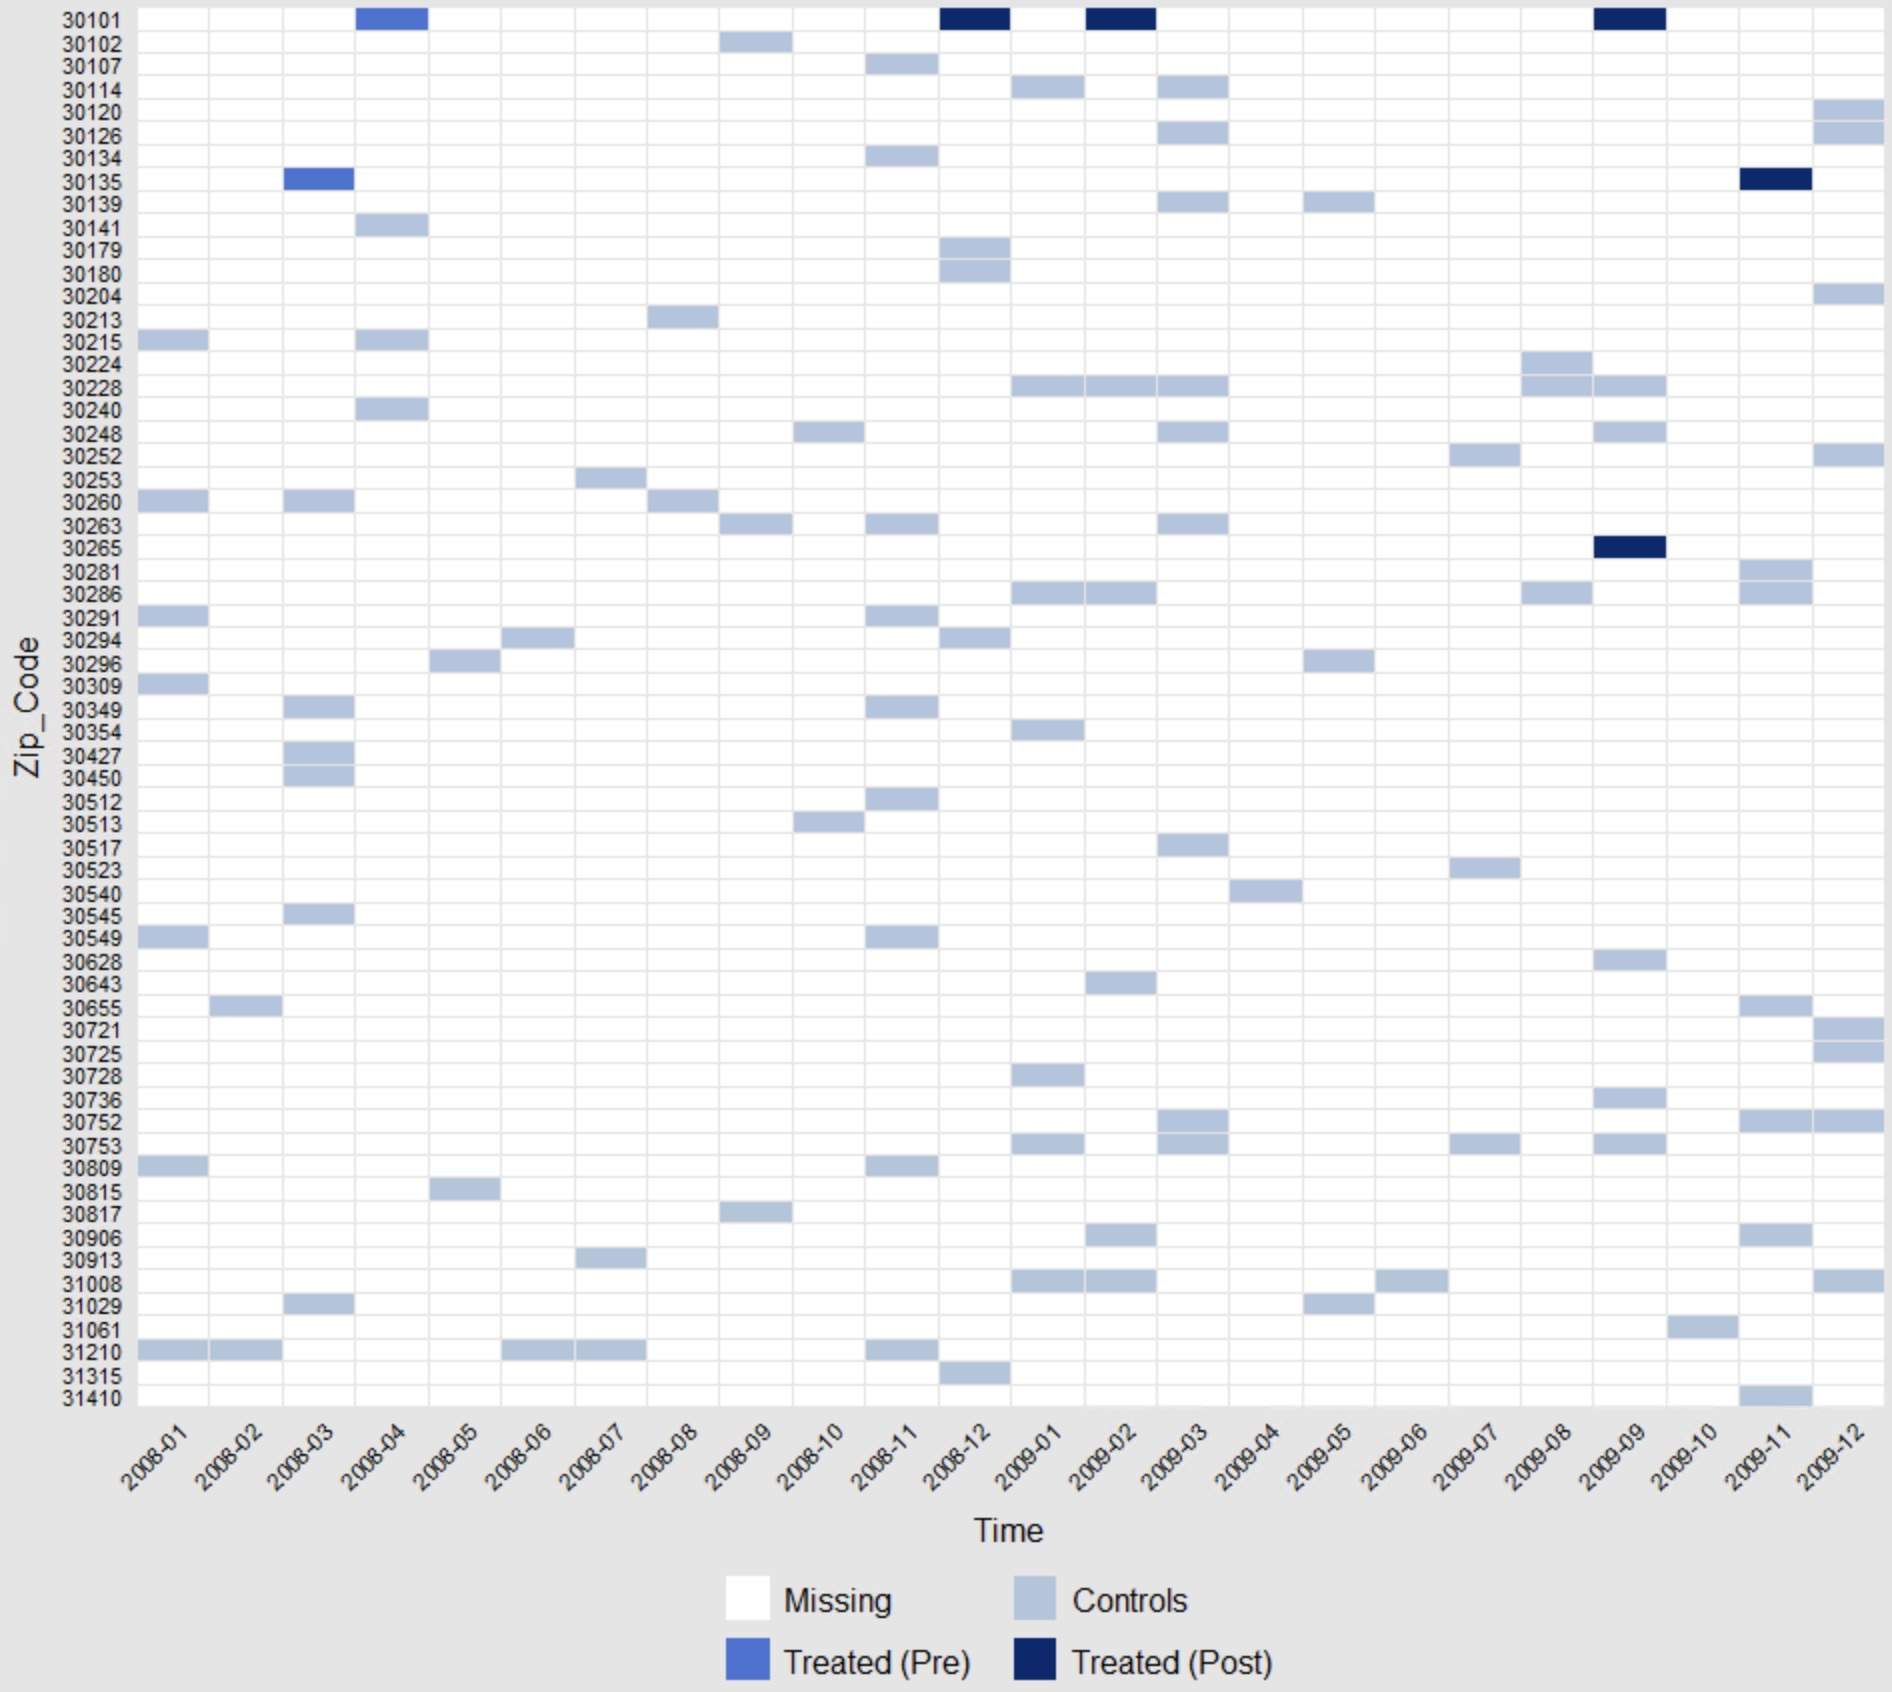
\includegraphics[scale = 0.23]{Panel View.jpg}
\end{figure}

With all restrictions stated above, we run the model on sales effect and search breadth and depth on both 0-mile data and 5-mile data, with outcome variable \texttt{AmazonTotalMonthlySales}, \texttt{AmazonPagesPerDollar} and \texttt{AmazonMinsPerDollar}, respectively. Table 25 shows the chosen number of latent variables and the \textit{Average Treatment effect on the Treated unit} (ATT) in each of the models.

\begin{table}[!h] \centering 
	\caption{Number of Latent Variables and the Averaage Treatment Effect for Amazon Data} 
	\label{tab:table25} 
	\resizebox{\columnwidth}{!}{
	\begin{tabular}{@{\extracolsep{1pt}}lD{.}{.}{-3} D{.}{.}{-3} D{.}{.}{-3} D{.}{.}{-3} D{.}{.}{-3} D{.}{.}{-3} } 
		\\[-1ex]\hline 
		\hline \\[-3ex] 
		%& \multicolumn{8}{c}{\textit{Dependent variable:}} \\ 
		%\cline{2-9} 
		%\\[-1.8ex] 
		& \multicolumn{2}{c}{AmazonTotalMonthlySales} & \multicolumn{2}{c}{AmazonPagesPerDollar} & 
		\multicolumn{2}{c}{AmazonMinsPerDollar}\\ 
		& \multicolumn{1}{c}{Amazon-0 Mile} & \multicolumn{1}{c}{Amazon-5 Miles} & \multicolumn{1}{c}{Amazon-0 Mile} & \multicolumn{1}{c}{Amazon-5 Miles} & \multicolumn{1}{c}{Amazon-0 Mile} & \multicolumn{1}{c}{Amazon-5 Miles} \\ 
		\\[-1.8ex] & \multicolumn{1}{c}{(1)} & \multicolumn{1}{c}{(2)} & \multicolumn{1}{c}{(3)} & \multicolumn{1}{c}{(4)} & \multicolumn{1}{c}{(5)} & \multicolumn{1}{c}{(6)} \\ 
		\hline \\[-3ex] 
		ATT & -0.863 & -0.248 & -0.210 & 0.024 & -0.293 &  -0.293\\ 
		& (1.316) & (0.229) & (18.580) & (0.211) & (1.038) & (1.067) \\ 
		\hline \\[-3ex] 
		r$^{*}$ & \multicolumn{1}{c}{0} & \multicolumn{1}{c}{0} & \multicolumn{1}{c}{1} & \multicolumn{1}{c}{0} & \multicolumn{1}{c}{0} & \multicolumn{1}{c}{0}  \\ 
		MSPE of r & \multicolumn{1}{c}{1.294} & \multicolumn{1}{c}{1.312} & \multicolumn{1}{c}{0.015} & \multicolumn{1}{c}{1.375} & \multicolumn{1}{c}{0.342} & \multicolumn{1}{c}{0.342} \\
		\hline
		\hline 
	\end{tabular} }
\end{table}

Codes for each of the models are listed below.
%\lstinputlisting[language=R, caption={Codes for GSC model}, label={codeGSC}, linerange={156-266}]{../GSC_part.R}


\pagebreak



%\subsection{Heckit Approach}

\subsection{PSM and LA-PSM}

%\subsection{Measurement Error Bias Correction}

\subsection{Causal Forest}
In this section we focus on transaction level data and our treated group is determined by using a 
a variable called \texttt{treatment} which takes value of 1 if \texttt{CCStorePresent} and \texttt{AfterStoreClosing} are 1 and takes value of 0 otherwise. \\

Codes for constructing treatment variable are listed below.
%\lstinputlisting[language=R, caption={Constructing  Treatment Variable}, label={lst:treatment_var}, linerange={117-129}]{../celik_beyza_causal_forest.R}

We first investigate the treatment effects on Amazon sales using the transactions within the zip code where a Circuit City store was closed. For each transaction $i=1, \cdots, n$, we observe a binary treatment indicator \texttt{treatment} ($W_i$), a real valued outcome \texttt{prod\_totprice} ($Y_i$), as well as 10 categorical covariates which are \texttt{hoh\_most\_education}, \texttt{census\_region}, \texttt{household\_size}, \texttt{hoh\_oldest\_age}, \texttt{children}, \texttt{racial\_background}, \texttt{connection\_speed}, \texttt{country\_of\_origin}, \texttt{prod\_category\_type} and \texttt{BBStorePresent}; and 4 real-valued covariates which are \texttt{pages\_viewed}, \texttt{duration}, \texttt{prod\_qty}, \texttt{household\_income}. We expanded out categorical random variables via one-hot encoding, thus resulting in covariates $X_i \in \mathbb{R}^p$  with $p = 38$. \\

We define causal effects via the potential outcomes model (Imbens and Rubin, 2015): For each sample
$i$, the potential outcomes denoted by $Y_i(0)$ and $Y_i(1)$ corresponding to the outcome we would have observed  if the $i$-th sample was in control or treatment group, and assume that we observe $Y_i =Y_i(Wi)$.
The average treatment effect is then defined as 
$\tau = \mathbb{E} [Y_i(1)-Y_i(0)]$, and the conditional average
treatment effect function is 
$\tau(x)=\mathbb{E}[ Y_i(1)-Y_i(0)\mid X_i] =x$ .\\

Codes for estimating treatment effects  on Amazon sales within the zip code where a Circuit City store was closed are listed below.
%\lstinputlisting[language=R, caption={Estimating Treatment Effects on Amazon Sales (Zero Mile) with Causal Forests}, label={lst:ama_cf_d1}, linerange={133-167}]{../celik_beyza_causal_forest.R}

We use the package \texttt{grf} to apply causal forest on our data and also to estimate the average treatment effect. the confidence interval for the average treatment effect is presented in Table \ref{tab:ama_cf1_ate}. Since the confidence interval includes zero we cannot conclude that treatment effect is significant.

\begin{table}[ht]
\caption{95\% CI for the ATE on Amazon Sales (Zero Mile Data)} 
\label{tab:ama_cf1_ate}
\vspace{1em}
\centering
\begin{tabular}{rrr}
  \hline
2.5\%  & Estimate & 97.5\% \\ 
  \hline
-19.28 & -7.68 & 3.92 \\ 
   \hline
\end{tabular}
\end{table}

%\lstinputlisting[language=R, caption={Estimating Treatment Effects on Amazon Sales (Zero Mile) with Causal Forests}, label={lst:ama_cf_d1}, linerange={170-173}]{../celik_beyza_causal_forest.R}

\begin{table}[ht]
\caption{95\% CI for the ATE on Amazon Pages Per Dollar (Zero Mile Data)} 
\vspace{1em}
\centering
\begin{tabular}{rrr}
  \hline
  2.5\%  & Estimate & 97.5\% \\ 
  \hline
 -39.25 & -23.62 & -7.98 \\ 
   \hline
\end{tabular}
\end{table}

\pagebreak
\section{Reference}
\setcitestyle{numbers} % set the citation style to ``numbers''.
\bibliographystyle{plainnat}
\bibliography{bobo}
% \bibliographystyle{plainnat}

Xu Y (2017) Generalized synthetic control method: Causal inference with interactive fixed effects models. \textit{Political Analysis.} 25(1):57-76

\end{document}
